\section{ Experiments and Results} \label{experiment}
We first conduct experiments with our custom-built 60 GHz mmWave imaging system to collect real 3D radar images. Our system and the experiment setup is shown in figure \ref{fig_exp}. Figure \ref{fig_real} is an example of the radar image we generate along with the scene it corresponds to. Although we can infer the overall shape of the Jeep from the radar image, the specularity effect is obvious, which makes breaks the car body into sparse clusters of reflectors.

\begin{figure}
	\centering
	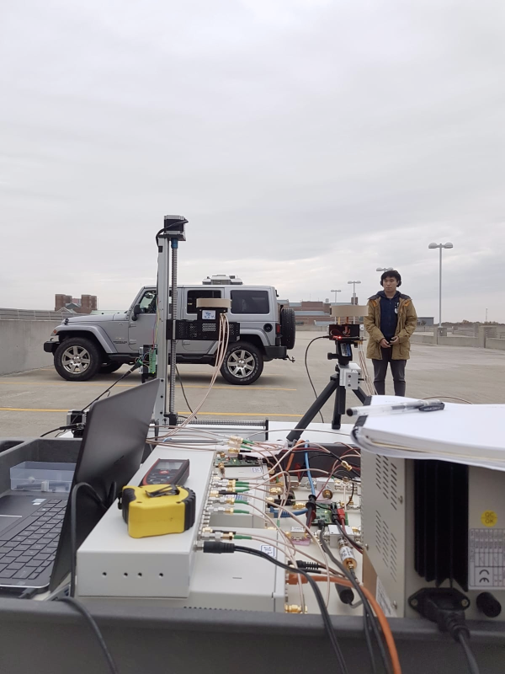
\includegraphics[width=6cm,height=8cm]{./figure/exp_2.png}\\
	\caption{Custom-built 60 GHz mmWave radar imaging system}
	\label{fig_exp}
\end{figure}

 Figure shows radar images we generate of a Jeep wrangler, from which we can clearly see that the specular reflection causes the car body to appear as sparse blobs. In other words, radar reflection off smooth objects might mainly towards an angle away from the receiver so as to disappears in the image.
 
\begin{figure}
	\centering
	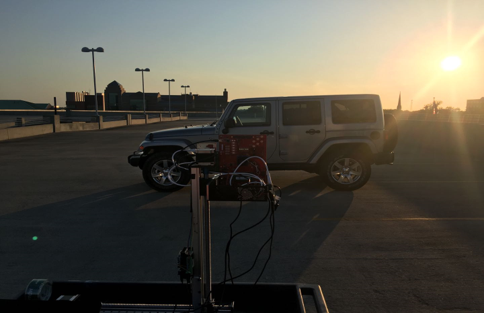
\includegraphics[width=7.5cm,height=4cm]{./figure/exp_1.png}\\
	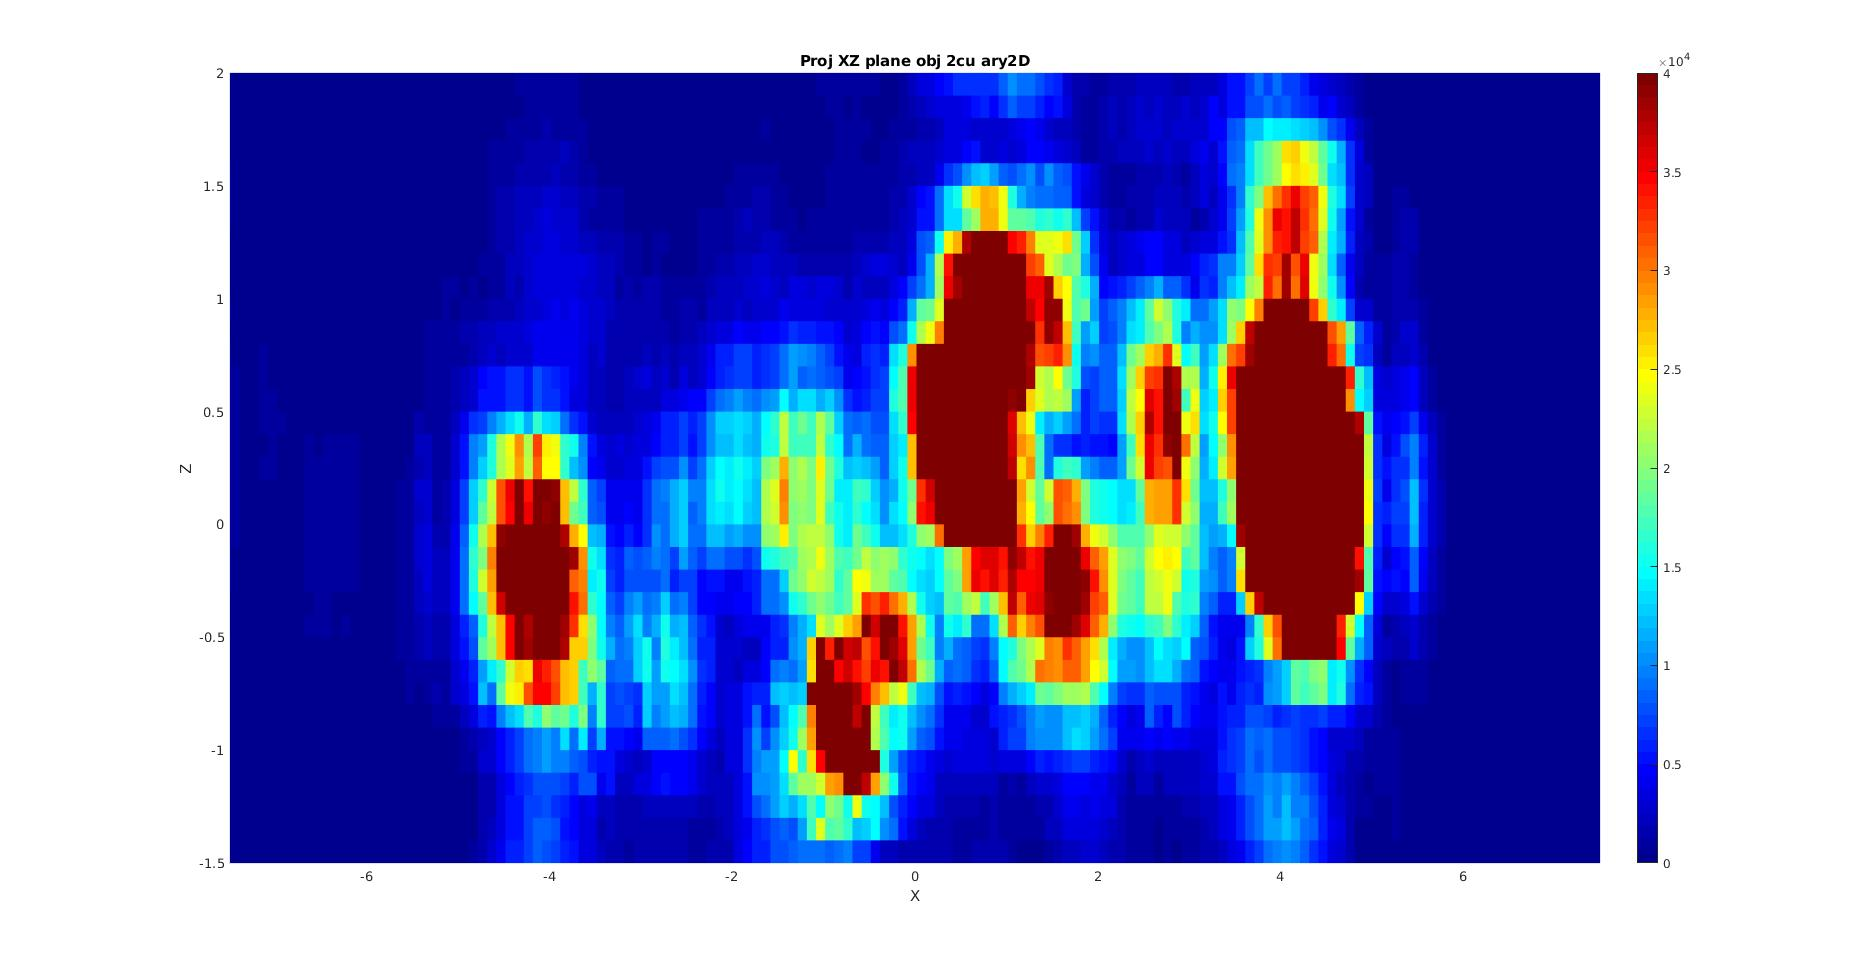
\includegraphics[width=9cm,height=6cm]{./figure/exp_1_img.jpg}
	\caption{Real radar image of a 2015 Jeep Wrangler}
	\label{fig_real}
\end{figure} 

Figure \ref{2D_synth} and \ref{3D_synth} demonstrate our 2D and 3D radar image synthesizing procedures. For 2D images generation, we start with video frames from the Cityscapes dataset ~\cite{cityscapes}, run trained Mask R-CNN model to detect and label objects ~\cite{rcnn}. It will also generate object masks which we will use to roughly recover the 3D scene and reflector model with. After that, we simulate radar signal and produce synthesized 2D radar images. At the same time, we extract a high quality images of objects from the camera pictures as the ground truth for our conditional GAN model.  For 3D image generation, we begin with 3D CAD models ~\cite{3Ddata}. We first transform the mesh format model into point reflectors by filling the mesh surfaces. Then we choose a reasonable point of view and transfer point reflector model into a spherical coordinate with the origin or our observing point. By selecting reflectors that are not blocked by others in front of them, we get the effective reflector distribution, and randomly choose a number of clusters to emulate the specularity effect. At the end, we implement the same radar simulation algorithms as the 2D case and generates realistic 3D radar images. 

\begin{figure}
	\centering
	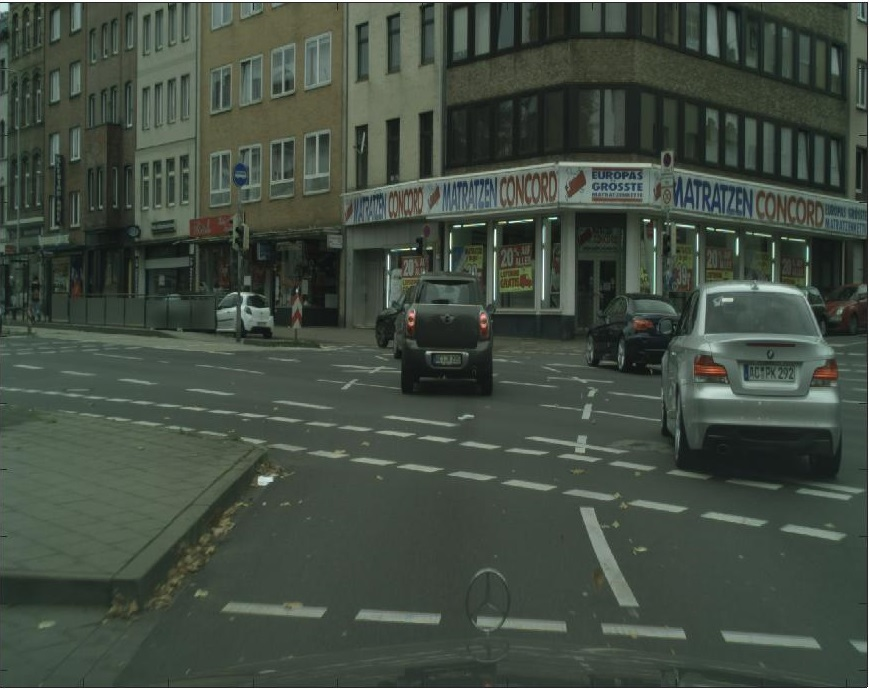
\includegraphics[width=8cm,height=4cm]{./figure/2d_origin.jpg}\\
	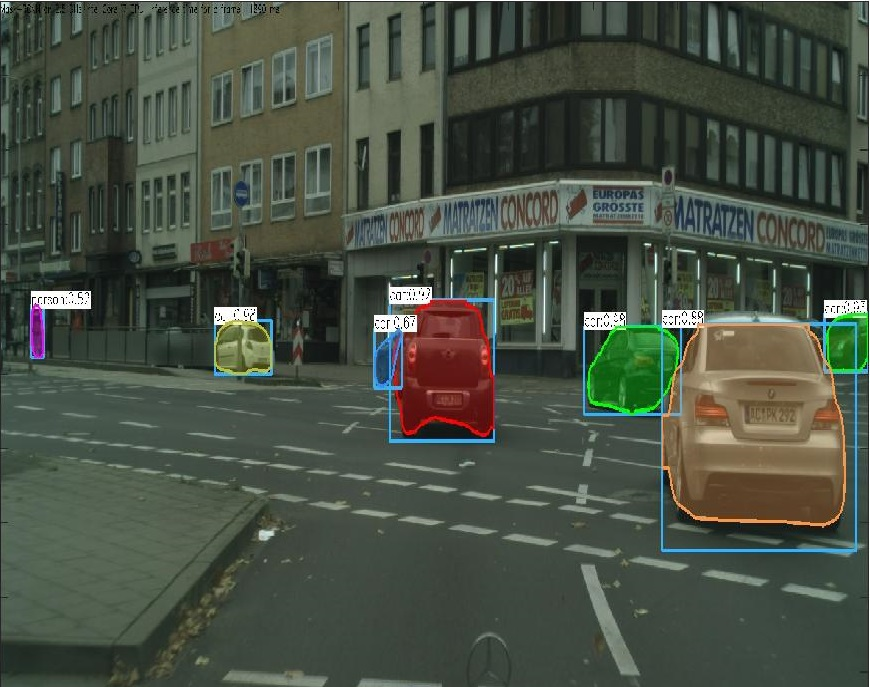
\includegraphics[width=8cm,height=4cm]{./figure/2d_detect.jpg}\\
	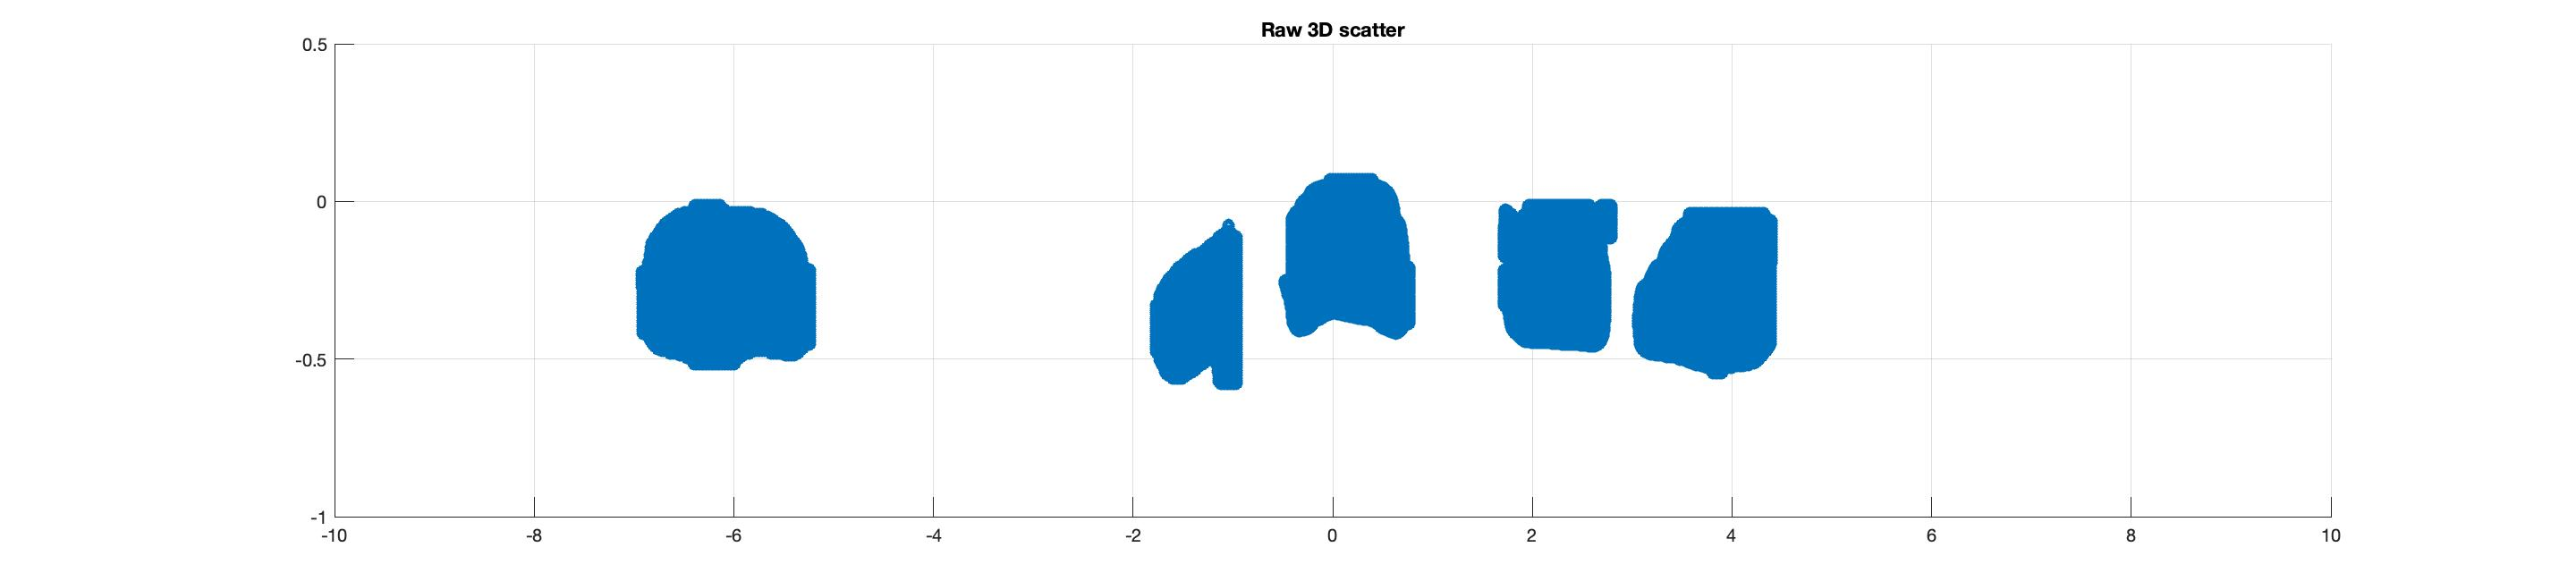
\includegraphics[width=9.5cm,height=4cm]{./figure/3d_cam.jpg}\\
	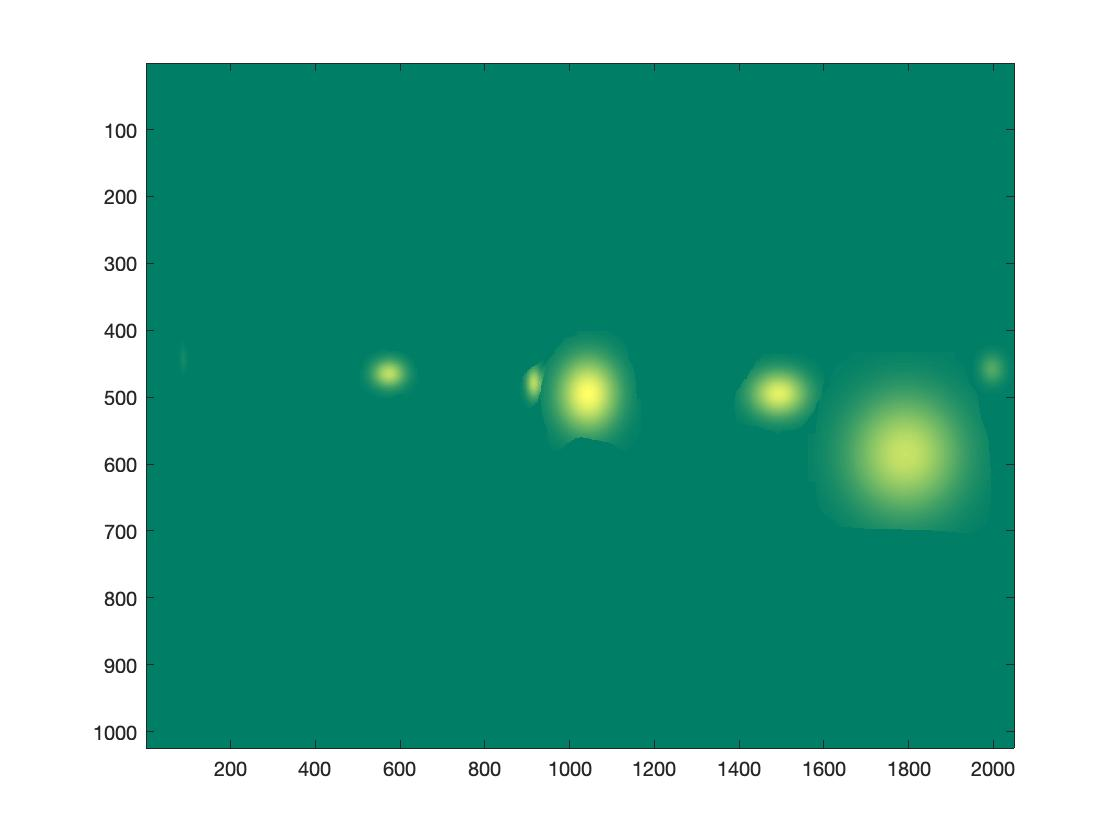
\includegraphics[width=8cm,height=4cm]{./figure/2d_blur.jpg}\\
	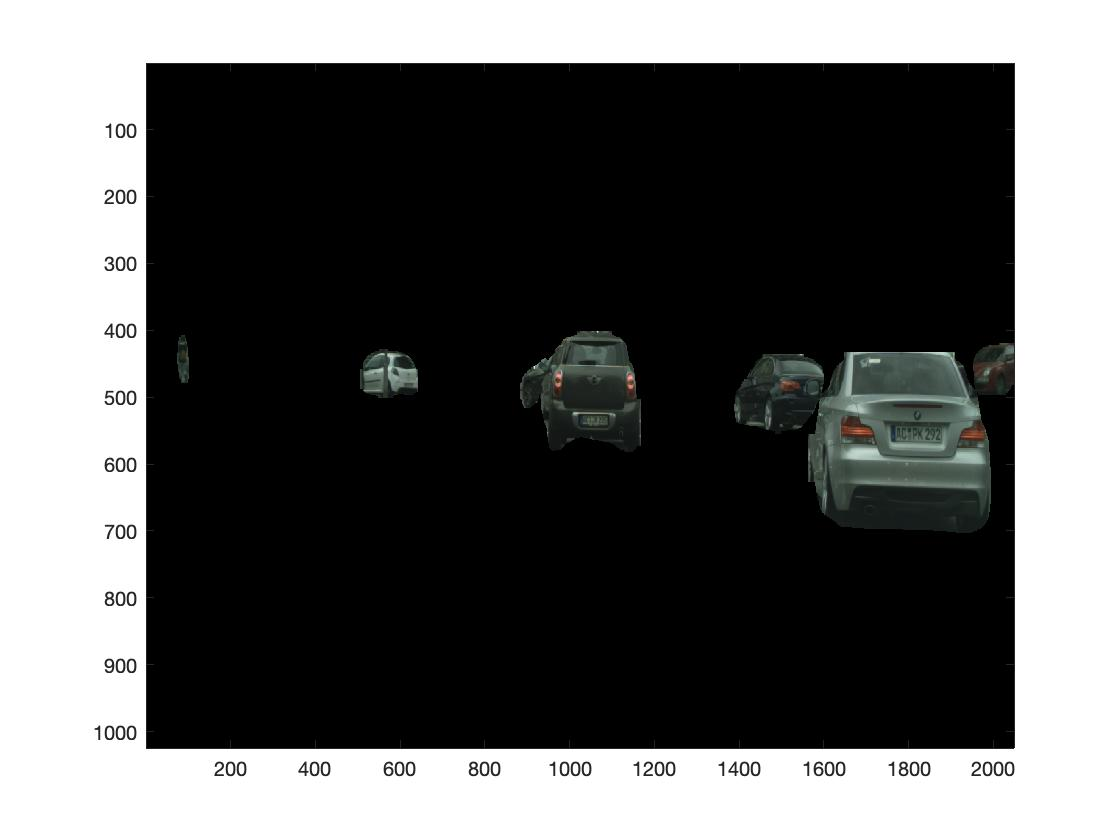
\includegraphics[width=8cm,height=4cm]{./figure/2d_select.jpg}\\
	\caption{2D radar image synthesizing procedure and result}
	\label{2D_synth}
\end{figure}

\begin{figure}
	\centering
	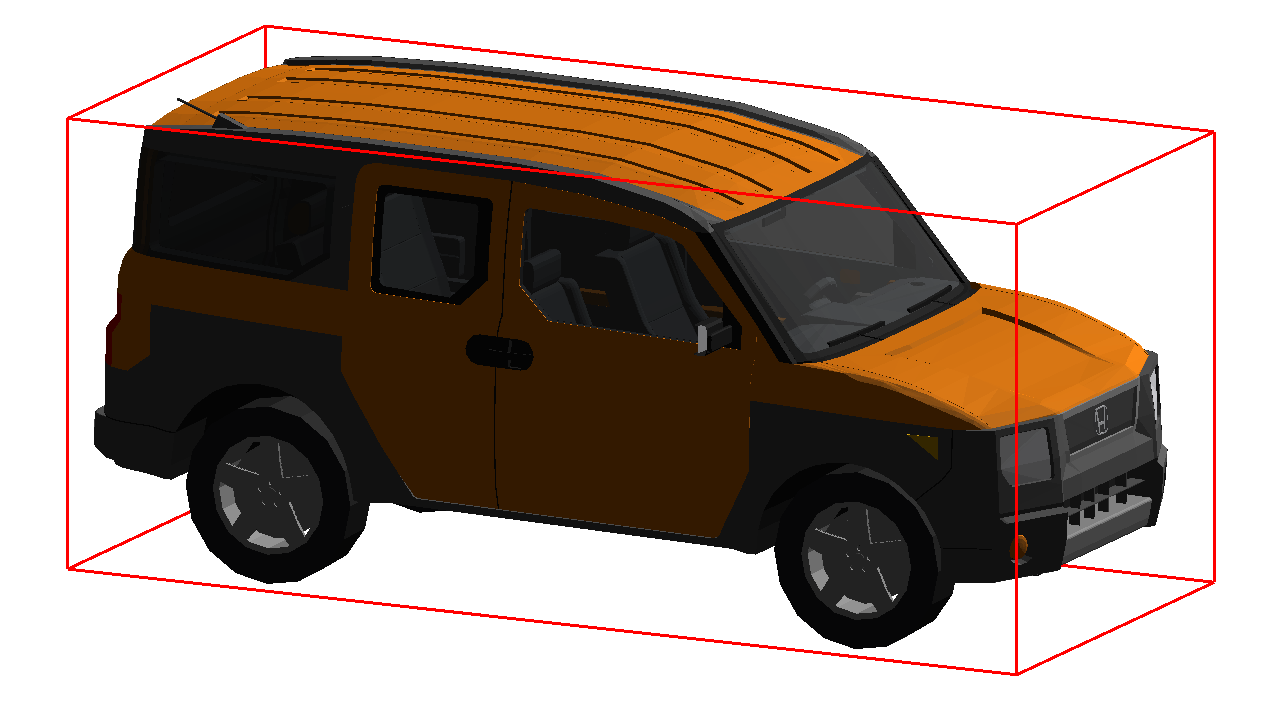
\includegraphics[width=7.5cm,height=4cm]{./figure/CAD.png}\\
	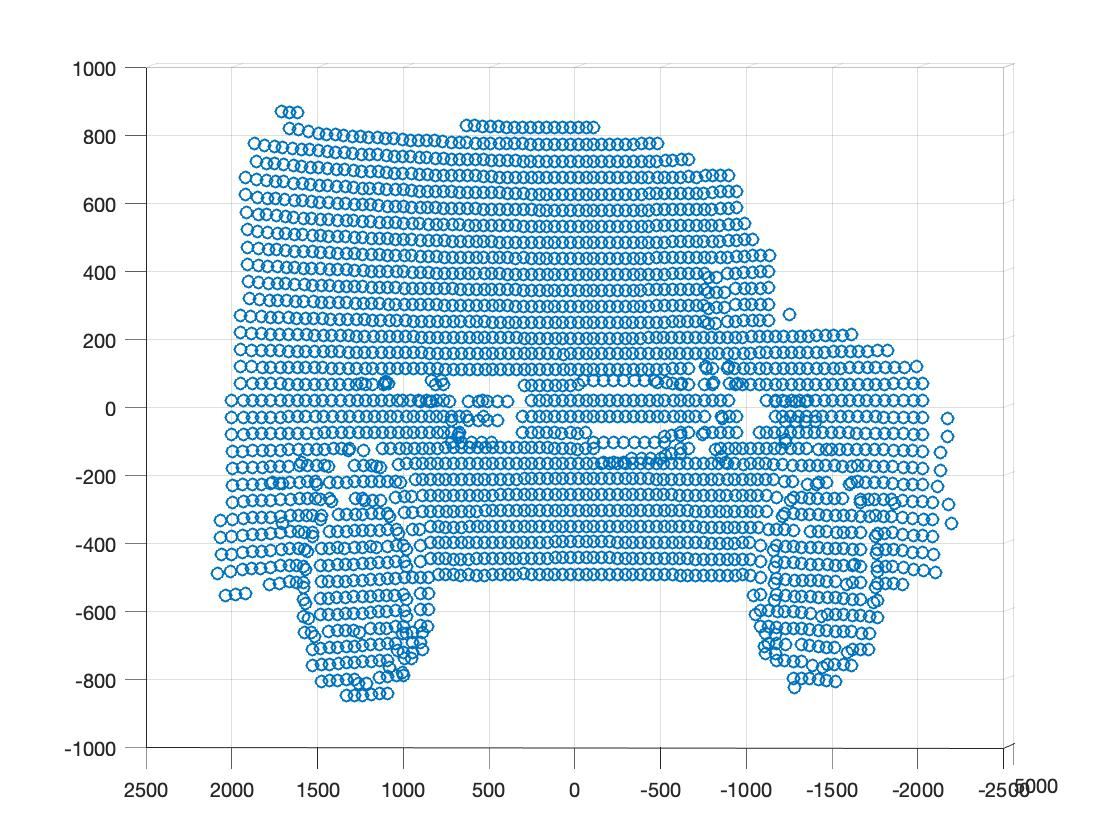
\includegraphics[width=9cm,height=6cm]{./figure/side.jpg}\\
	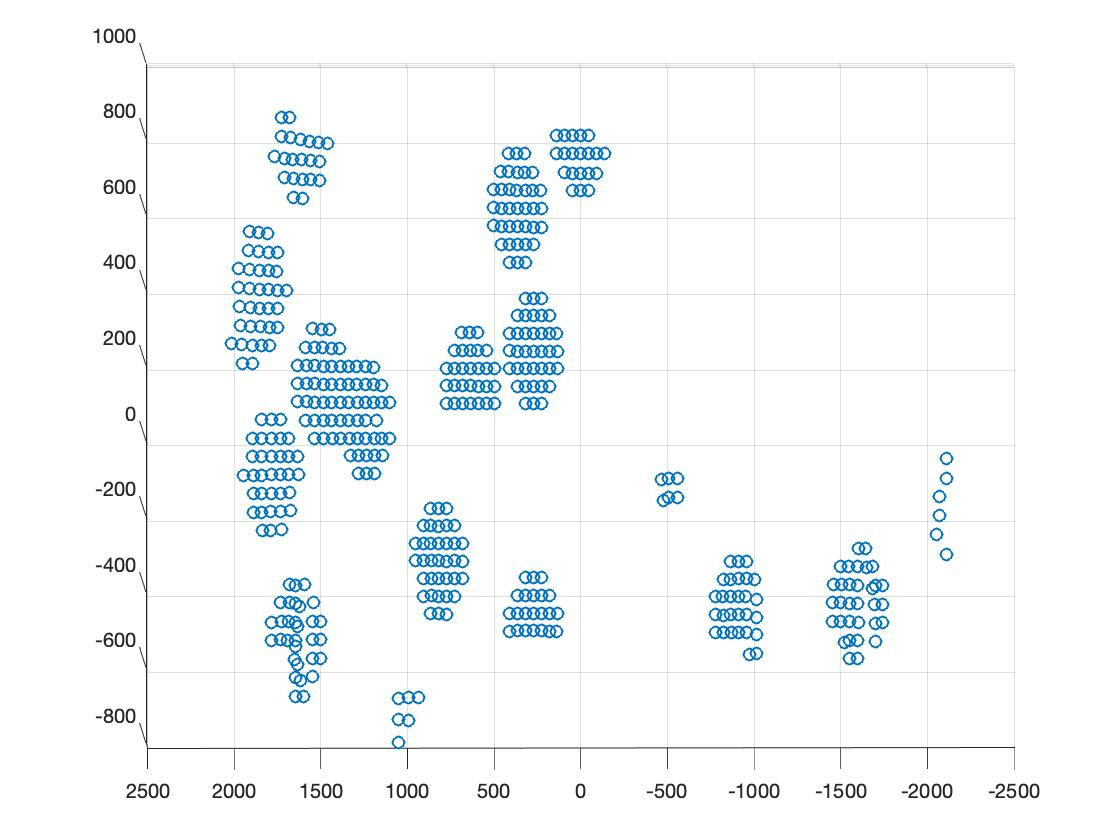
\includegraphics[width=9cm,height=6cm]{./figure/specular.jpg}\\
	\caption{Custom-built 60 GHz mmWave radar imaging system}
	\label{3D_synth}
\end{figure}

For our experiments, we ran our data one NVIDIA Tesla K80 GPU available on Google Cloud using CUDA 9.0 and PyTorch 0.4, along with a local Pascal GTX 1080 GPU using CUDA 10.0 and PyTorch 1.0. We used 1056 images of size $256 \times 256$ as for training, and 452 images for testing. The training phase takes about 11 hours to finish if the complete training dataset is used.

%\begin{figure*}[h]
%	\def\tabularxcolumn#1{m{#1}}
%
%	\begin{tabularx}{\linewidth}{| c | c | c |}
%	
%		\begin{tabular}{cc}
%			\subfloat{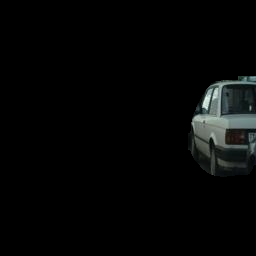
\includegraphics[width=3.7cm, height=1.85cm]{./figure/126_real_B}}\\ 
%			ground truth \\
%		\end{tabular}
%		&
%		\begin{tabular}{cc}
%			\subfloat{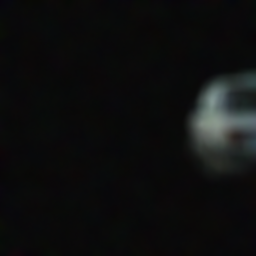
\includegraphics[width=3.7cm, height=1.85cm]{./figure/126_real_A}}\\  
%			blurred image\\
%		\end{tabular}
%		&
%		\begin{tabular}{cc}
%			\subfloat{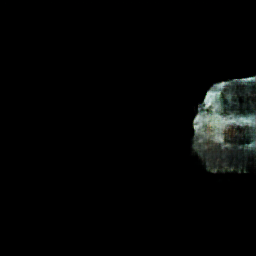
\includegraphics[width=3.7cm, height=1.85cm]{./figure/126_fake_B}}\\ 
%			generated image \\
%		\end{tabular}
%	\end{tabularx}	
%	\caption{Result from the toy experiment. The GAN has successfully estimated the boundary of the car.}\label{fig1}
%\end{figure*}

\begin{figure}
	\centering
	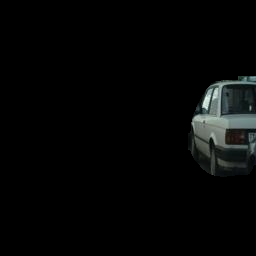
\includegraphics[width=5.4cm, height=2.7cm]{./figure/126_real_B}\\
	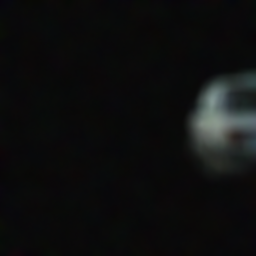
\includegraphics[width=5.4cm, height=2.7cm]{./figure/126_real_A}\\
	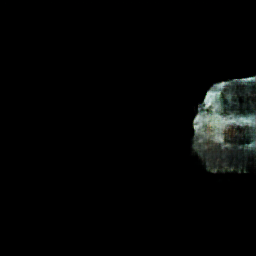
\includegraphics[width=5.4cm, height=2.7cm]{./figure/126_fake_B}\\
	\caption{Result from the first experiment. The GAN has succesfully estimated the boundary of the car.}\label{fig1}
\end{figure}

The first experiment we ran on the GPU was a toy example using blurred images as input. We took the images of cars, added some Gaussian noise and convolved the image with a two-dimensional $sinc$ function. We fed these images as input, and the original images to the network as ground truth. the results showed that the network is able to restore the boundaries of the cars with a high accuracy. The problem with this implementation was that the image was not gray-scaled, and we did not go through a precise simulation according the to underlying physics of mmWave radars to generate the images. The purpose of this step was to evaluate the feasibility of our idea of restoring the boundaries using GANs on a high level. The results from this experiments are shown in figure \ref{fig1}. It can be seen that the boundary of the car has been fairly accurately reconstructed. It is also noteworthy that the GAN was able to restore the side mirror of the car successfully, although there is no side mirror visible point in GAN. 

\begin{figure*}
	\def\tabularxcolumn#1{m{#1}}
	\begin{tabularx}{\linewidth}{| c | c | c | c | }
%		\begin{tabular}{cc}
%			\subfloat{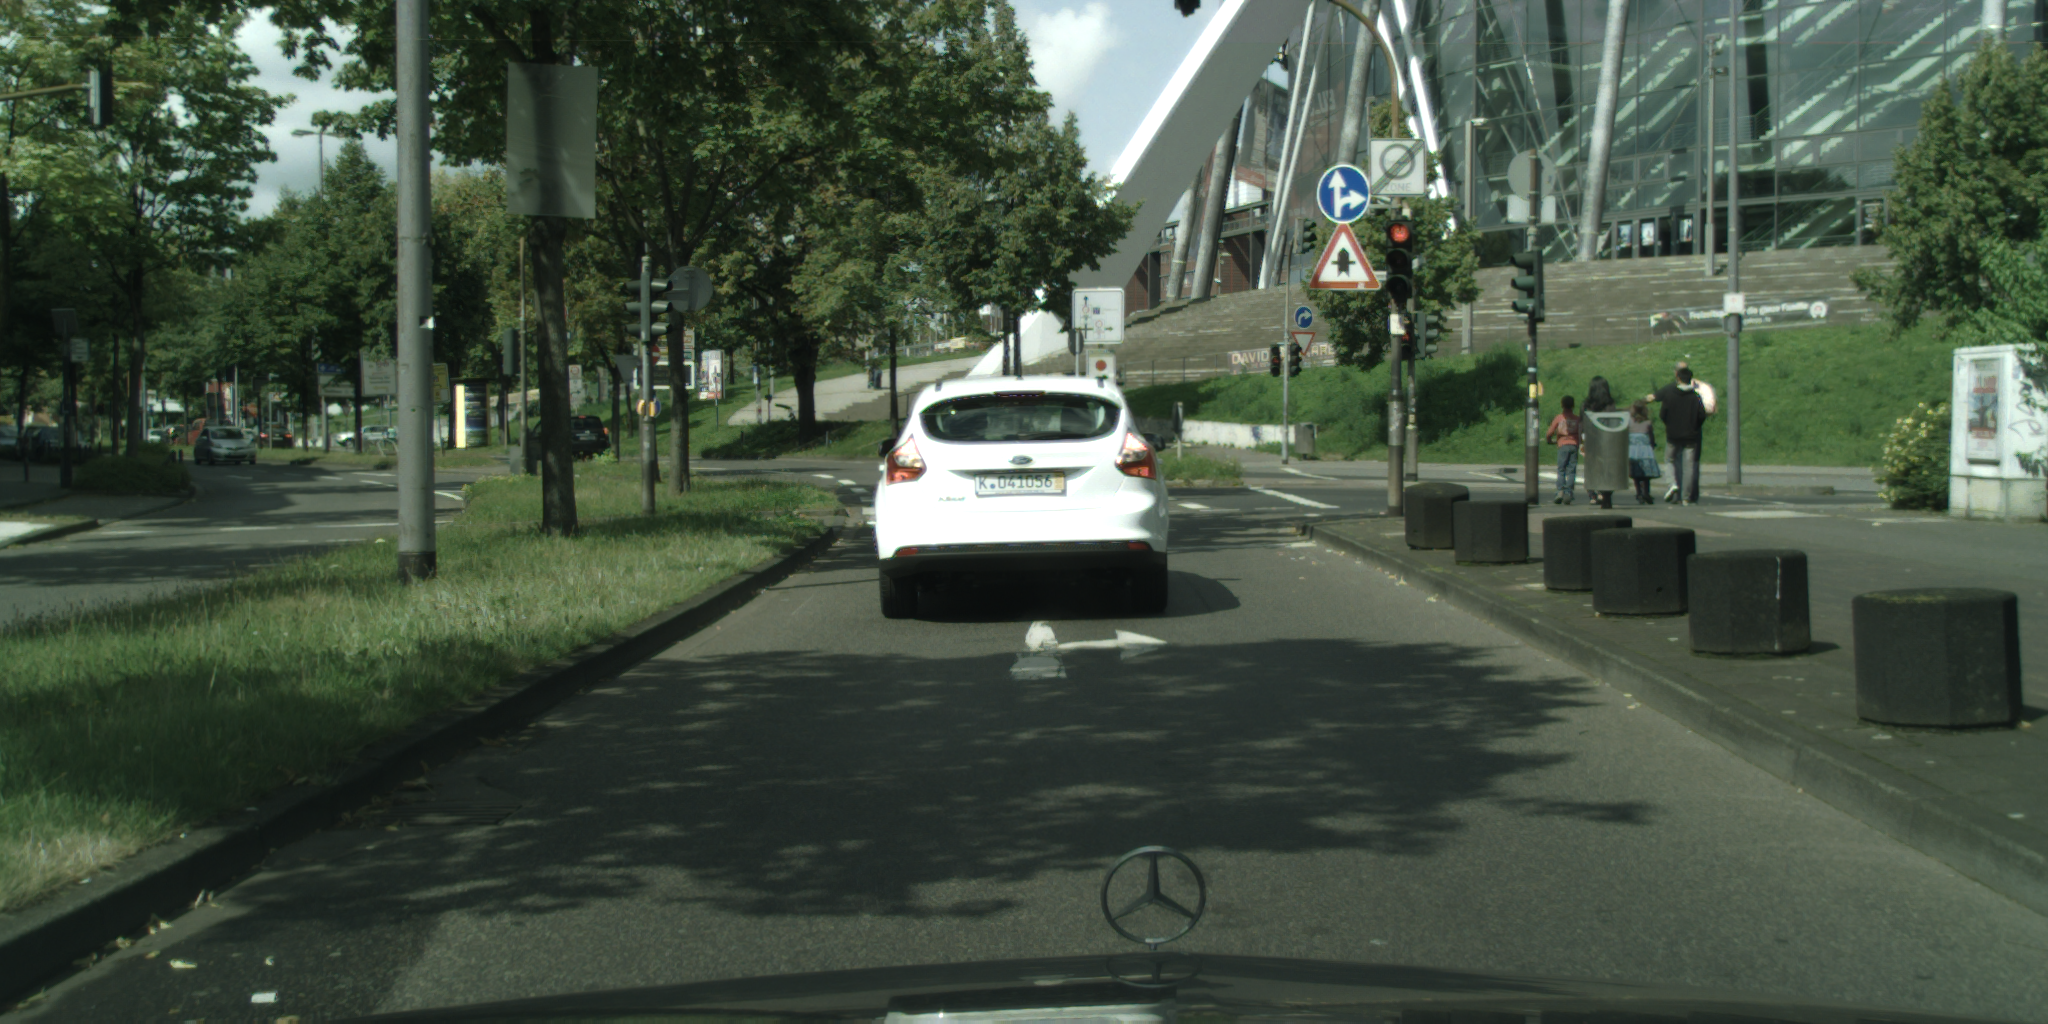
\includegraphics[width=3.7cm, height=1.85cm]{./figure/cologne_000011_000019_leftImg8bit}}\\ 
%			\subfloat{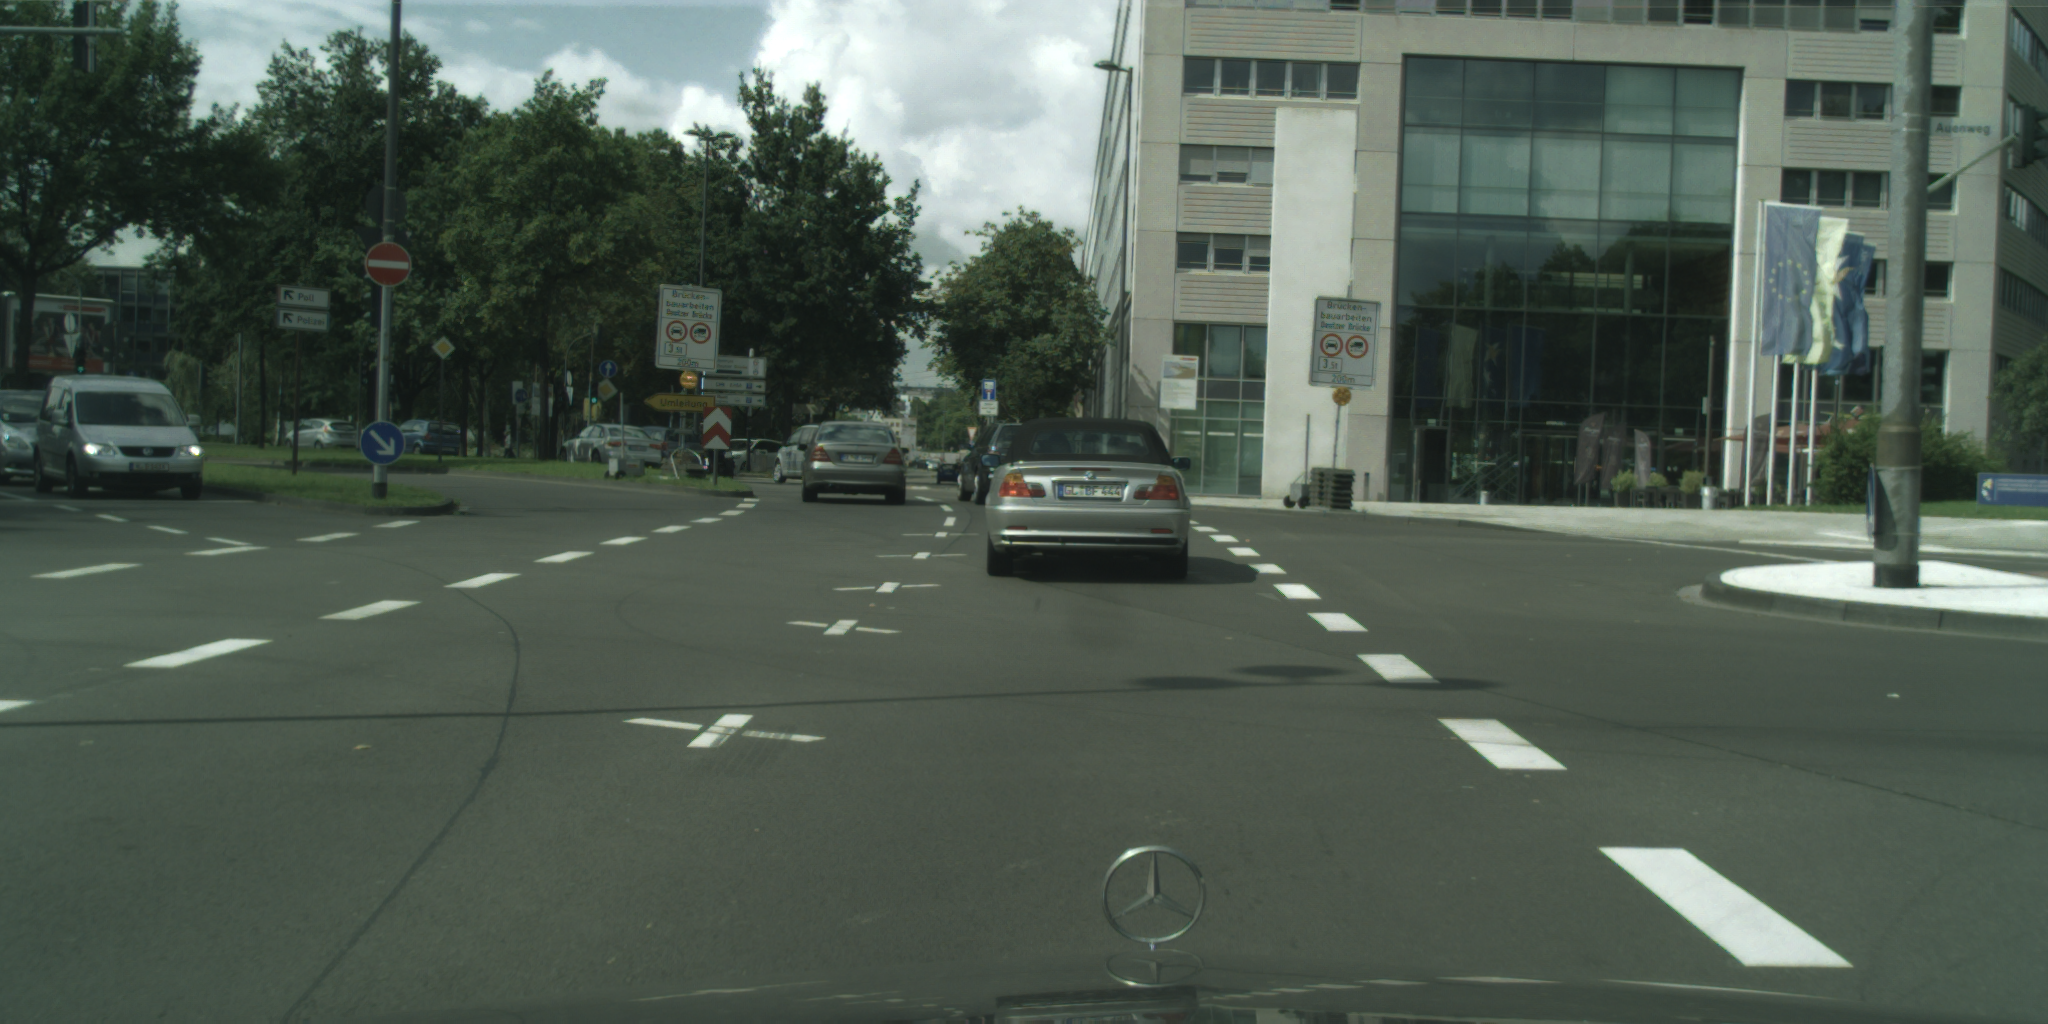
\includegraphics[width=3.7cm, height=1.85cm]{./figure/cologne_000013_000019_leftImg8bit.png}}\\
%			\subfloat{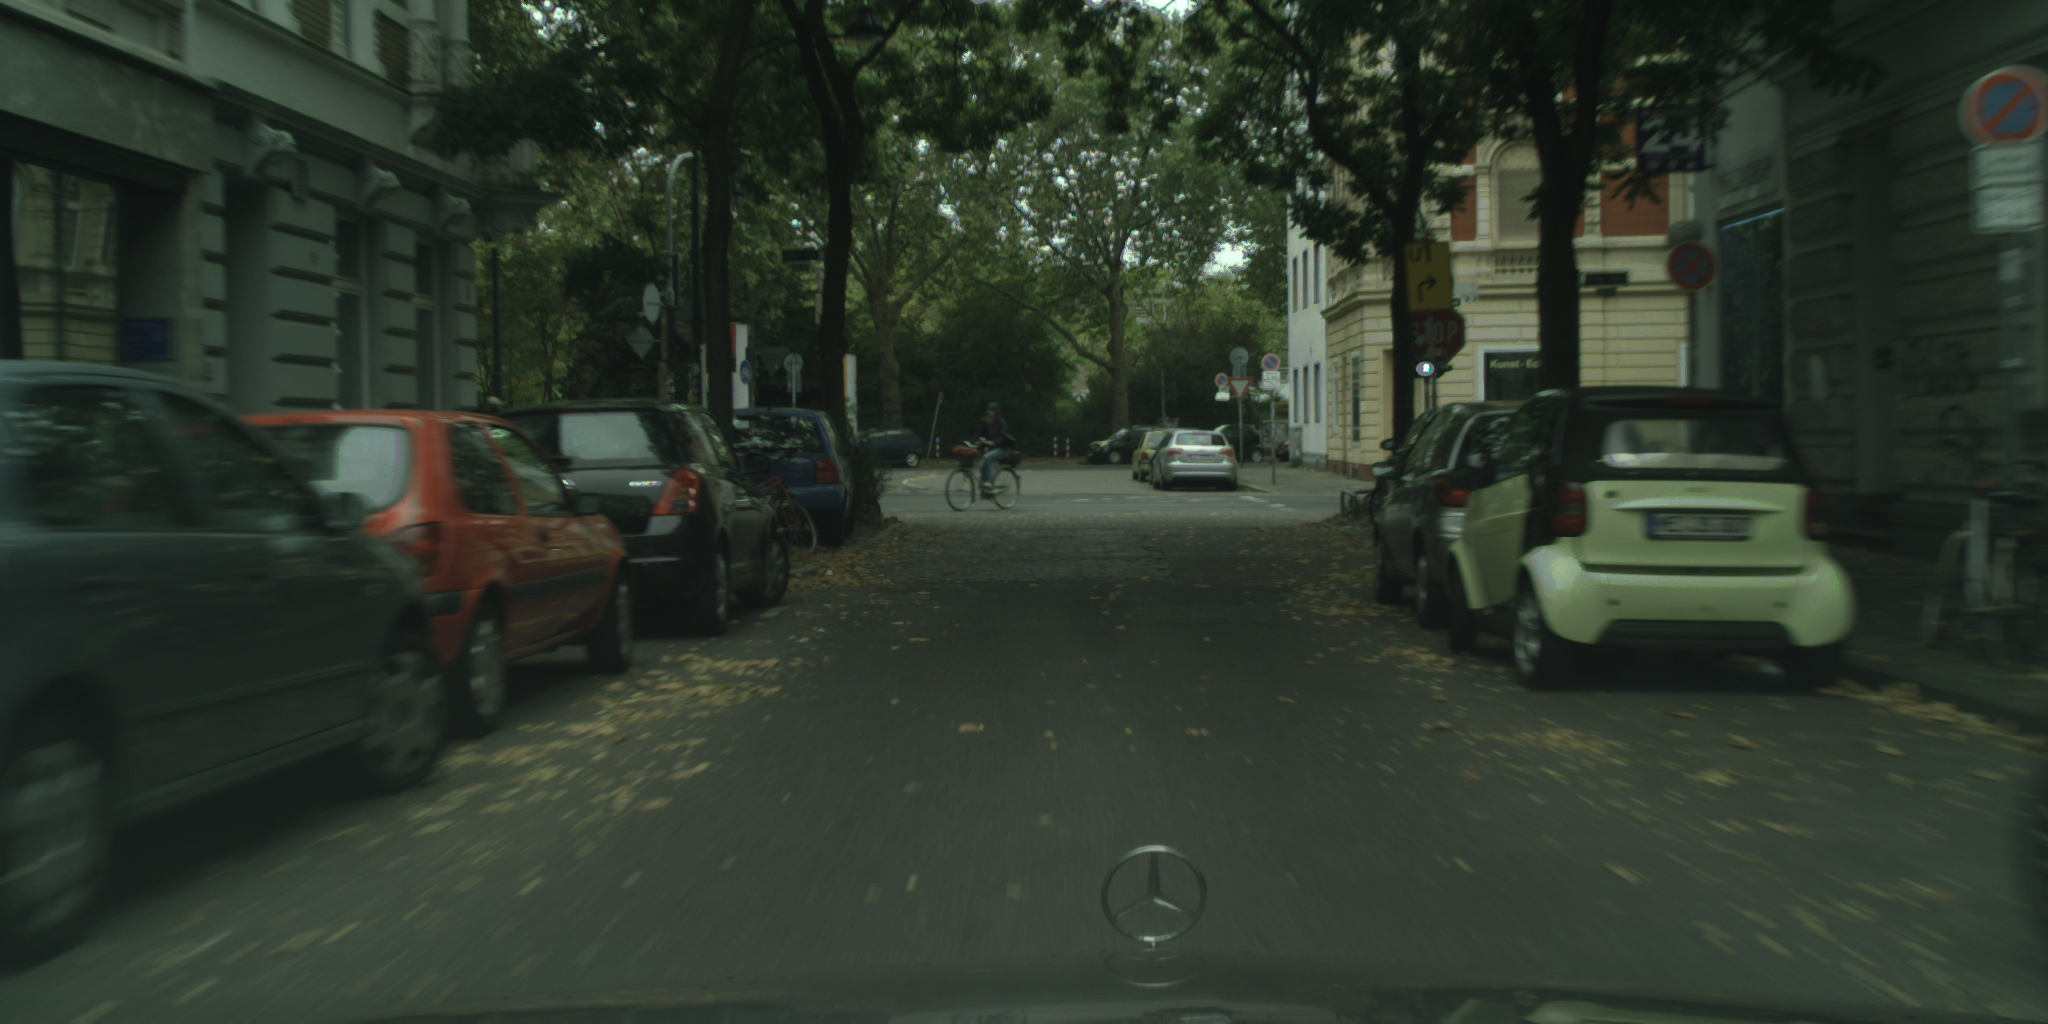
\includegraphics[width=3.7cm, height=1.85cm]{./figure/dusseldorf_000008_000019_leftImg8bit.png}}\\ 
%			\subfloat{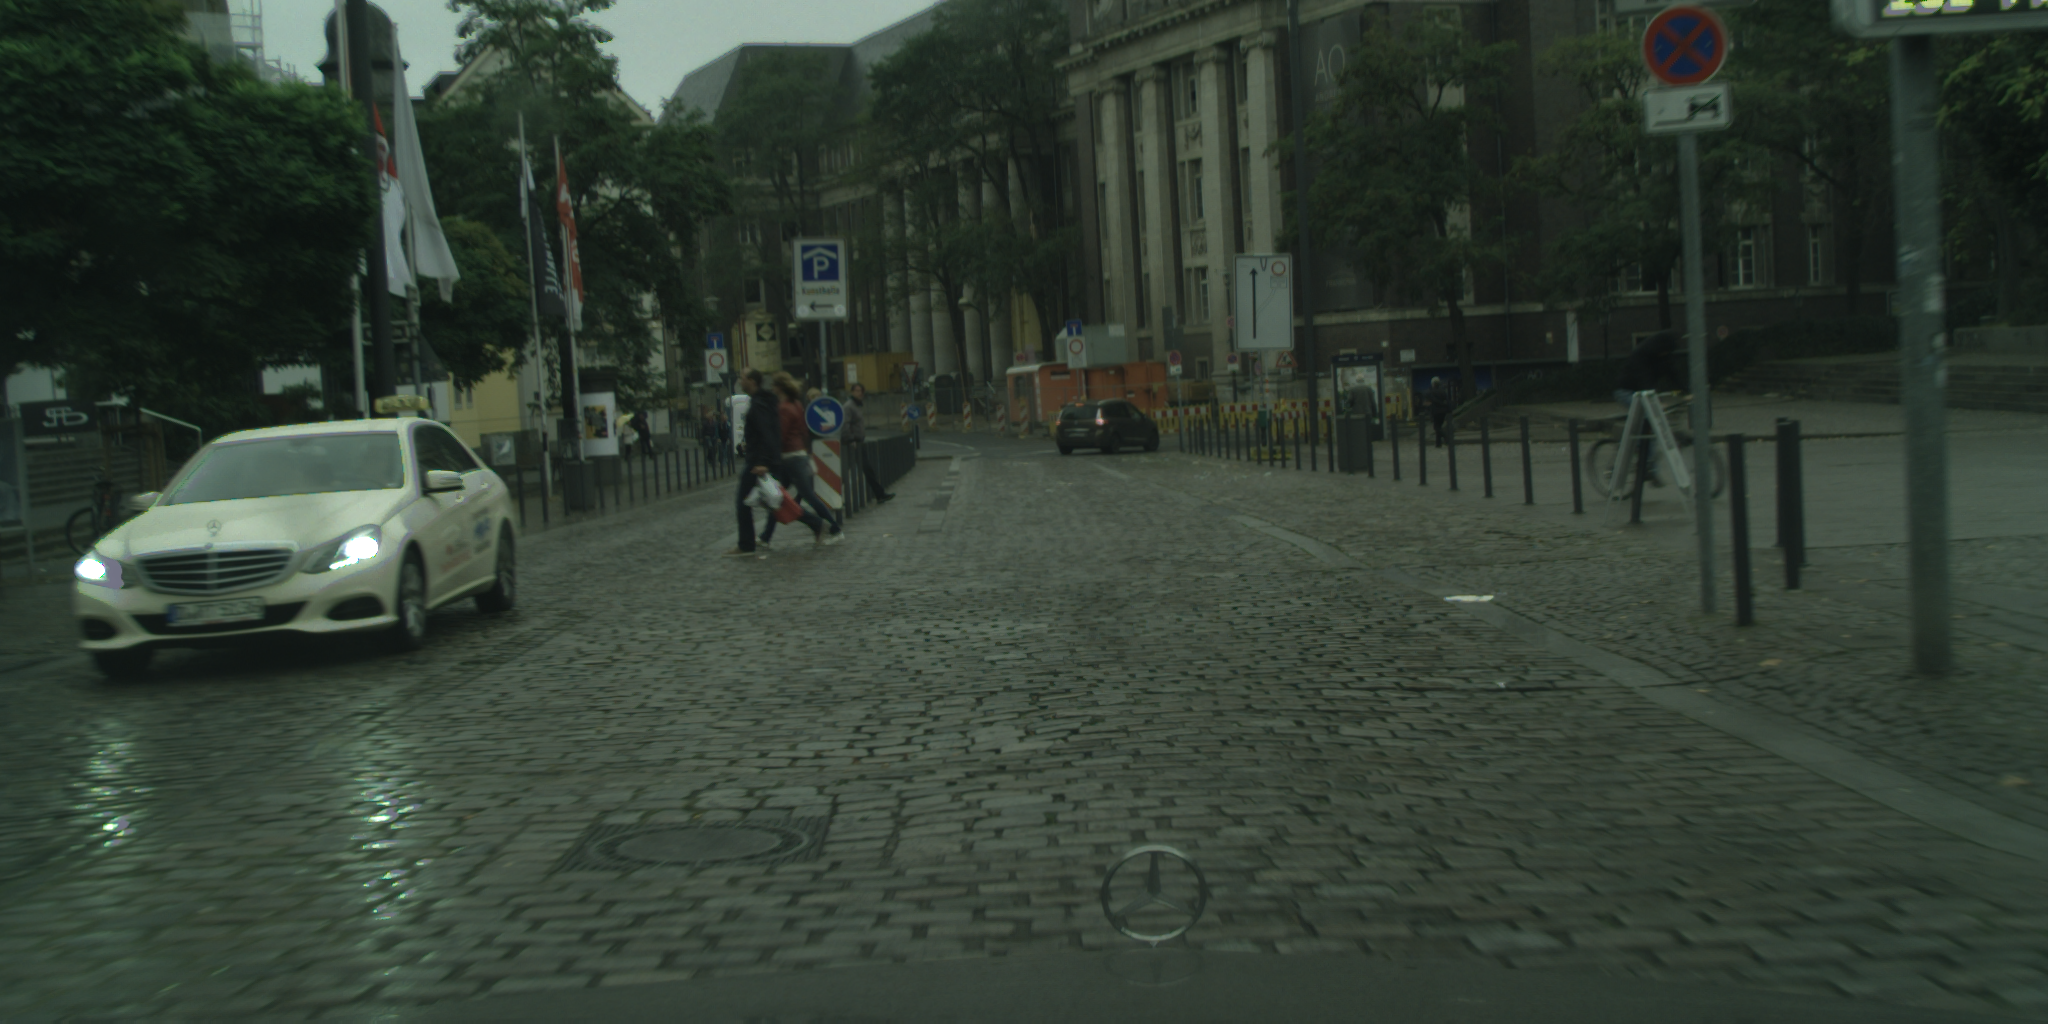
\includegraphics[width=3.7cm, height=1.85cm]{./figure/dusseldorf_000040_000019_leftImg8bit.png}}\\
%			\subfloat{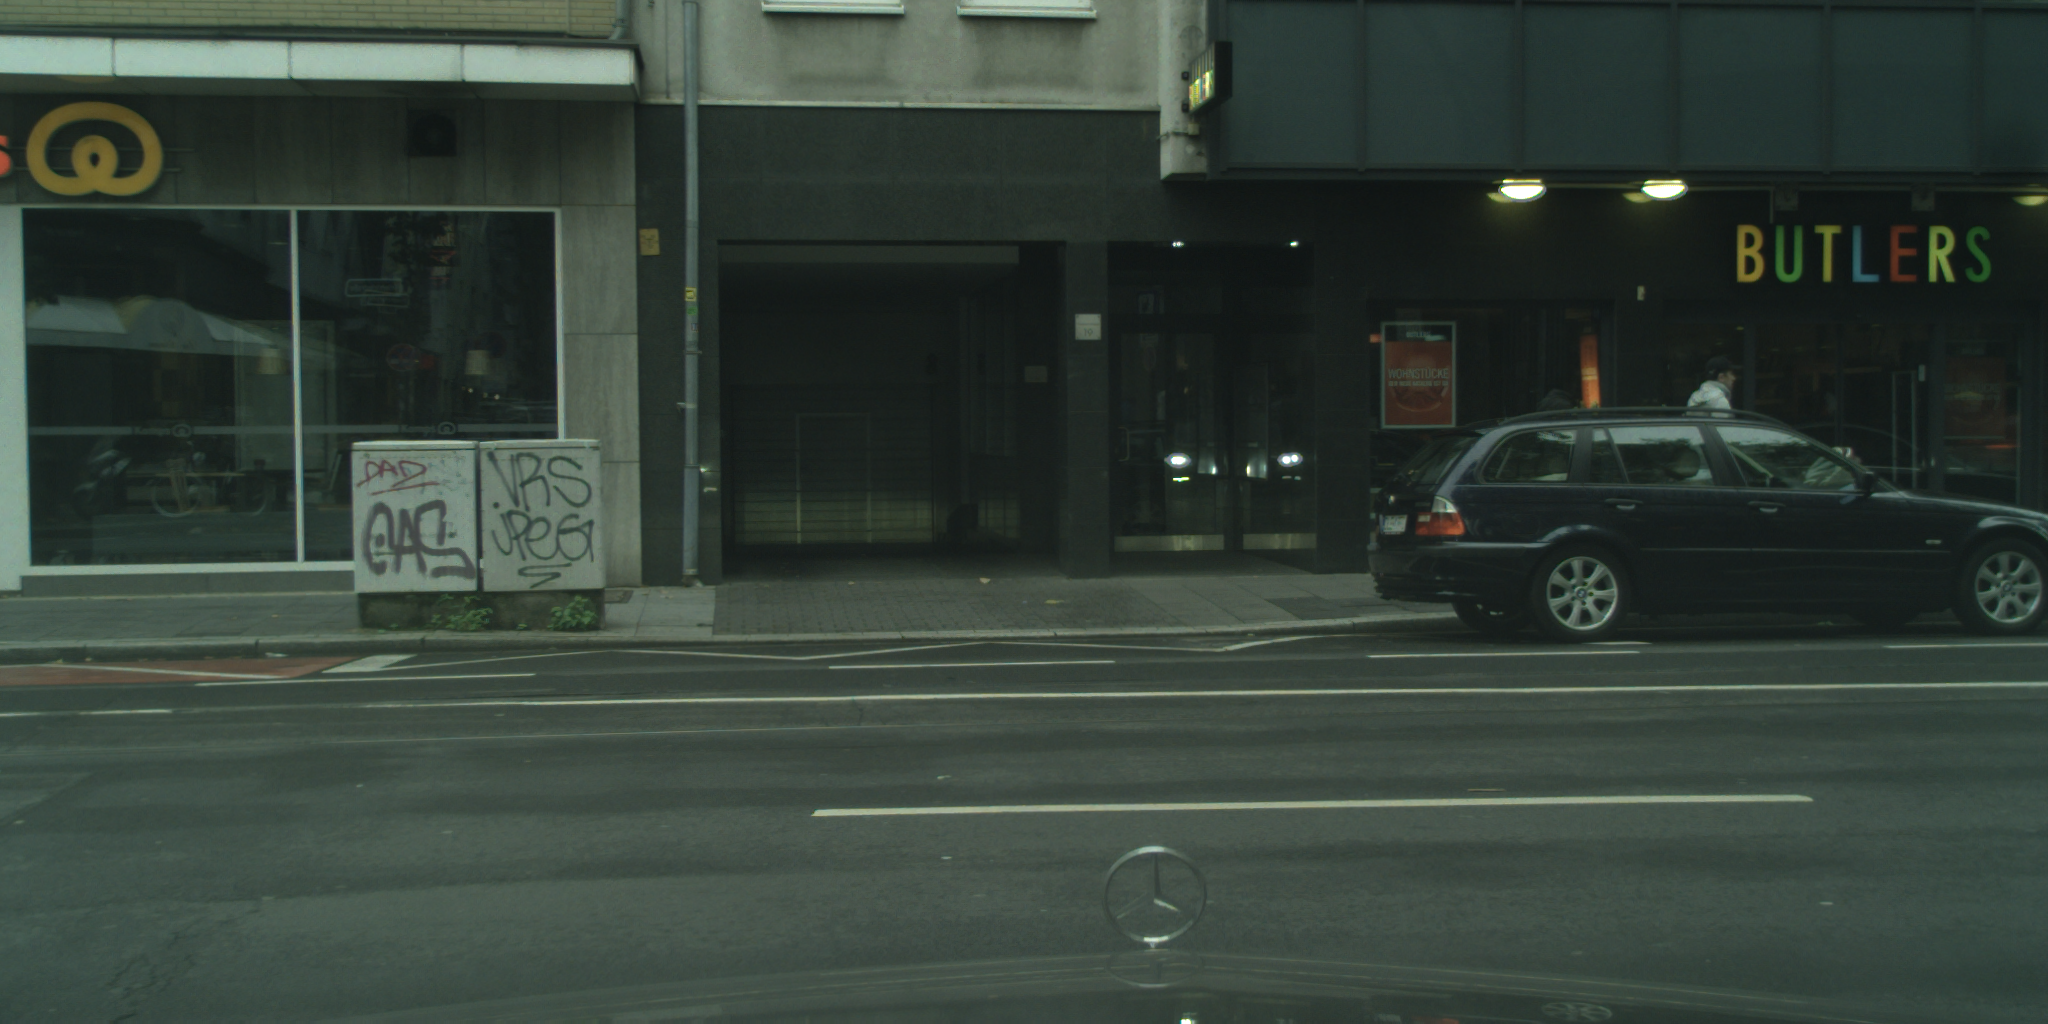
\includegraphics[width=3.7cm, height=1.85cm]{./figure/dusseldorf_000088_000019_leftImg8bit.png}}\\ 
%			(a) original image \\
%		\end{tabular}
%		&
		\begin{tabular}{cc}
			\subfloat{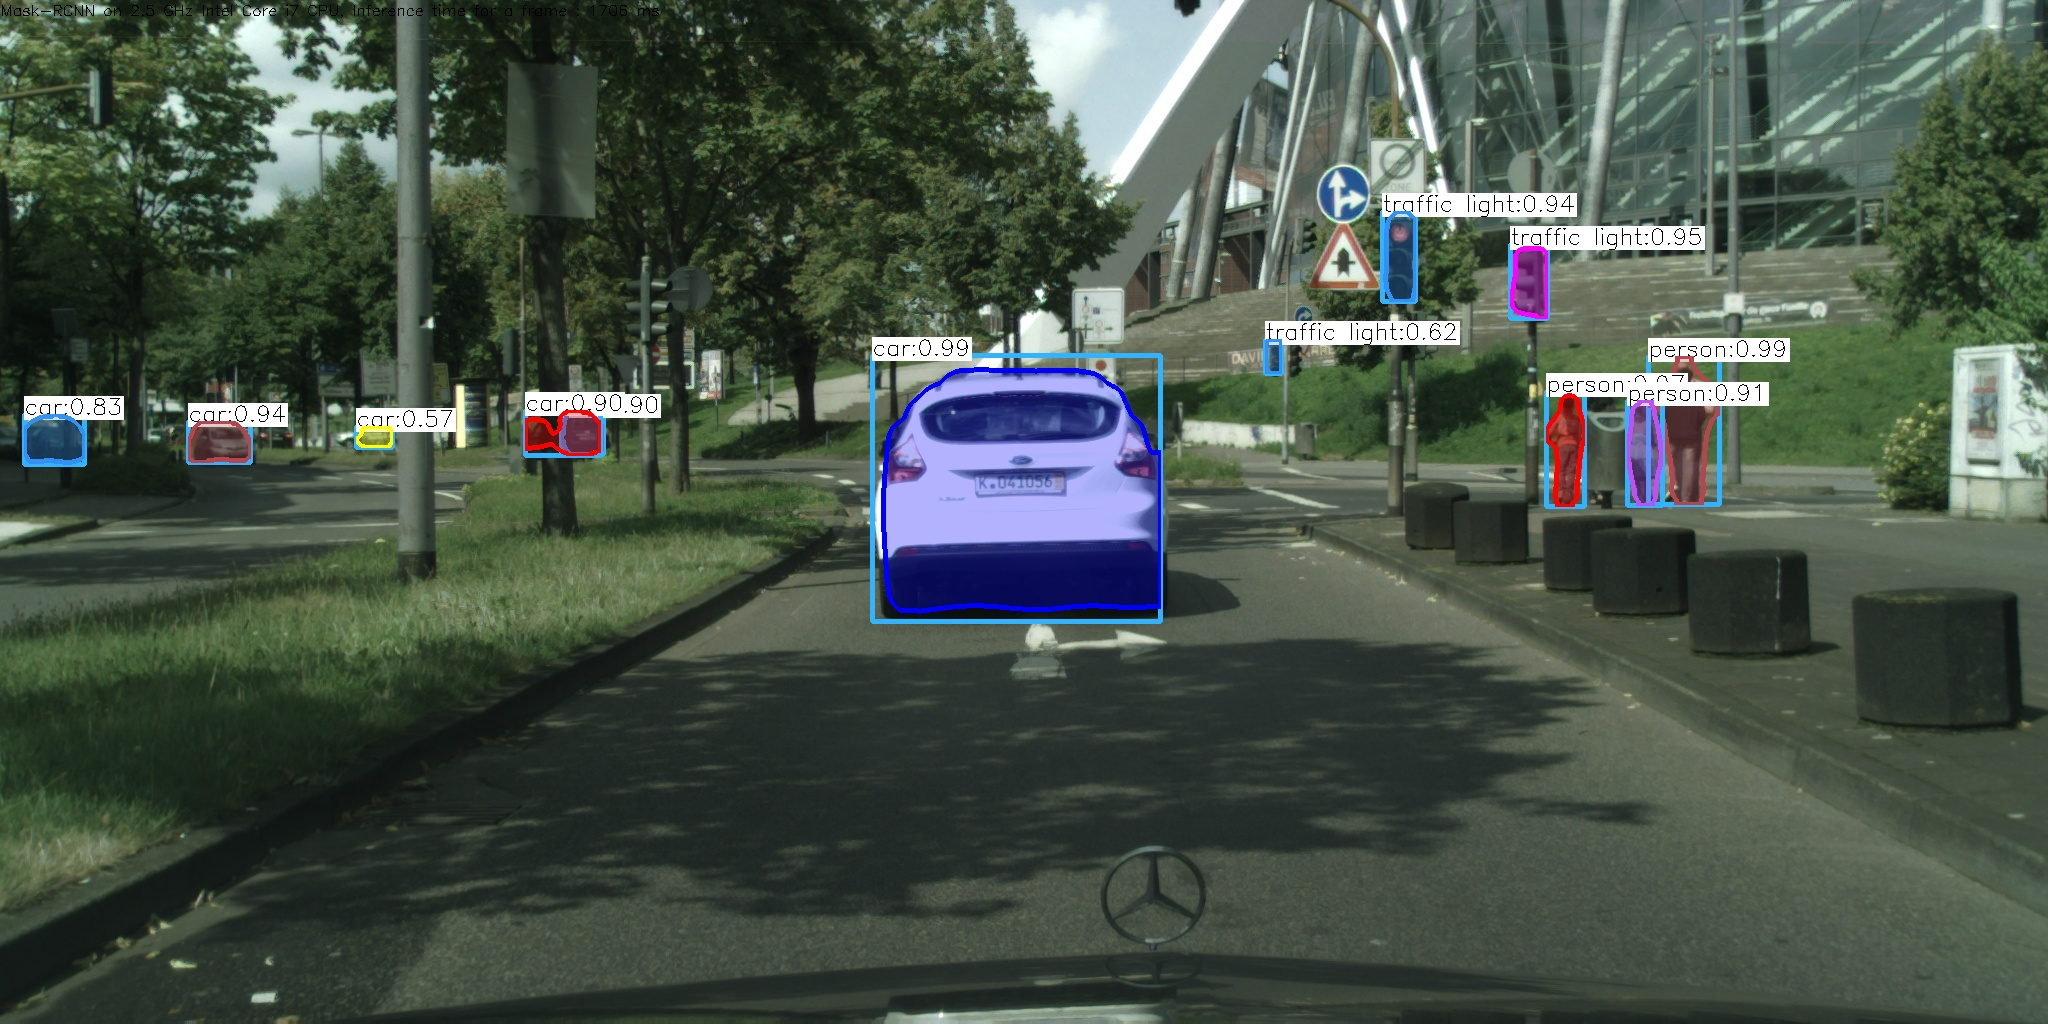
\includegraphics[width=3.7cm, height=1.85cm]{./figure/cologne_000011_000019_leftImg8bit_mask_rcnn_out_py.jpg}}\\ 
			\subfloat{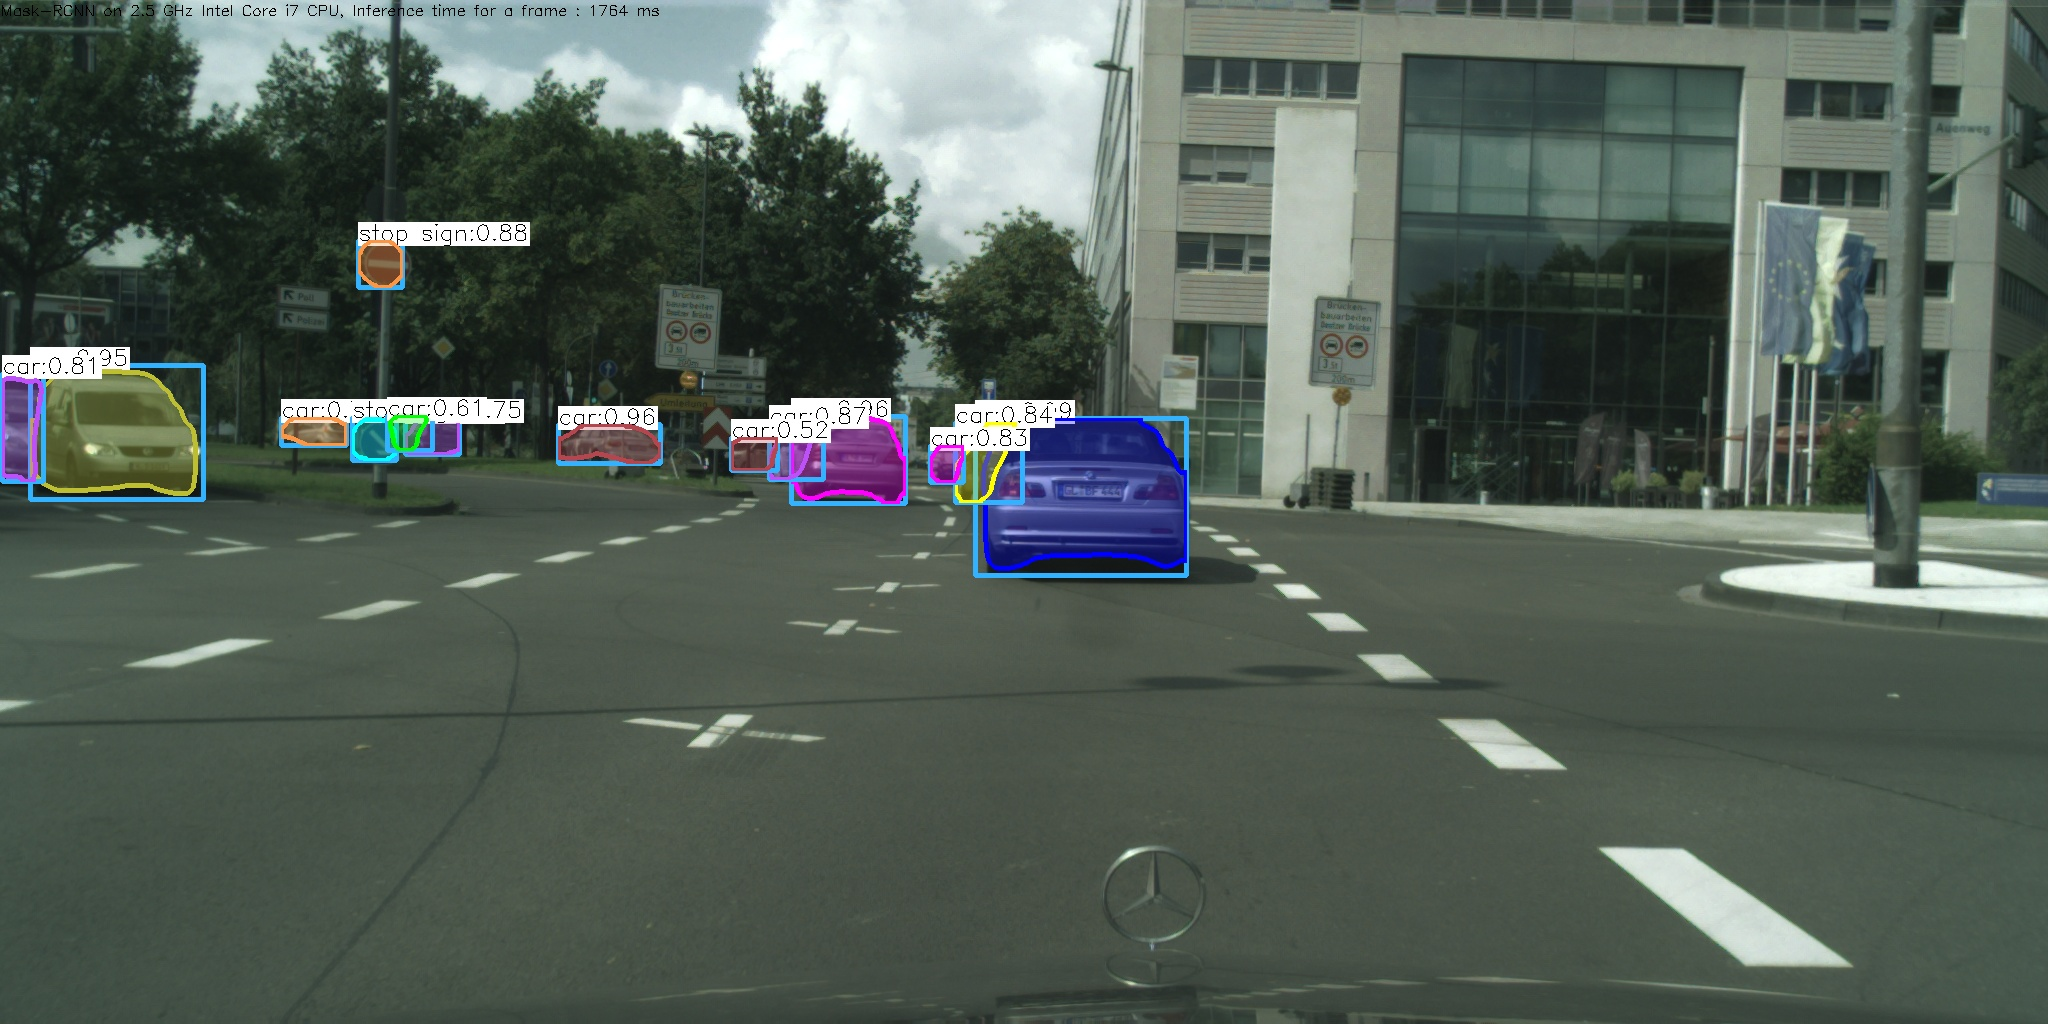
\includegraphics[width=3.7cm, height=1.85cm]{./figure/cologne_000013_000019_leftImg8bit_mask_rcnn_out_py.jpg}}\\
			\subfloat{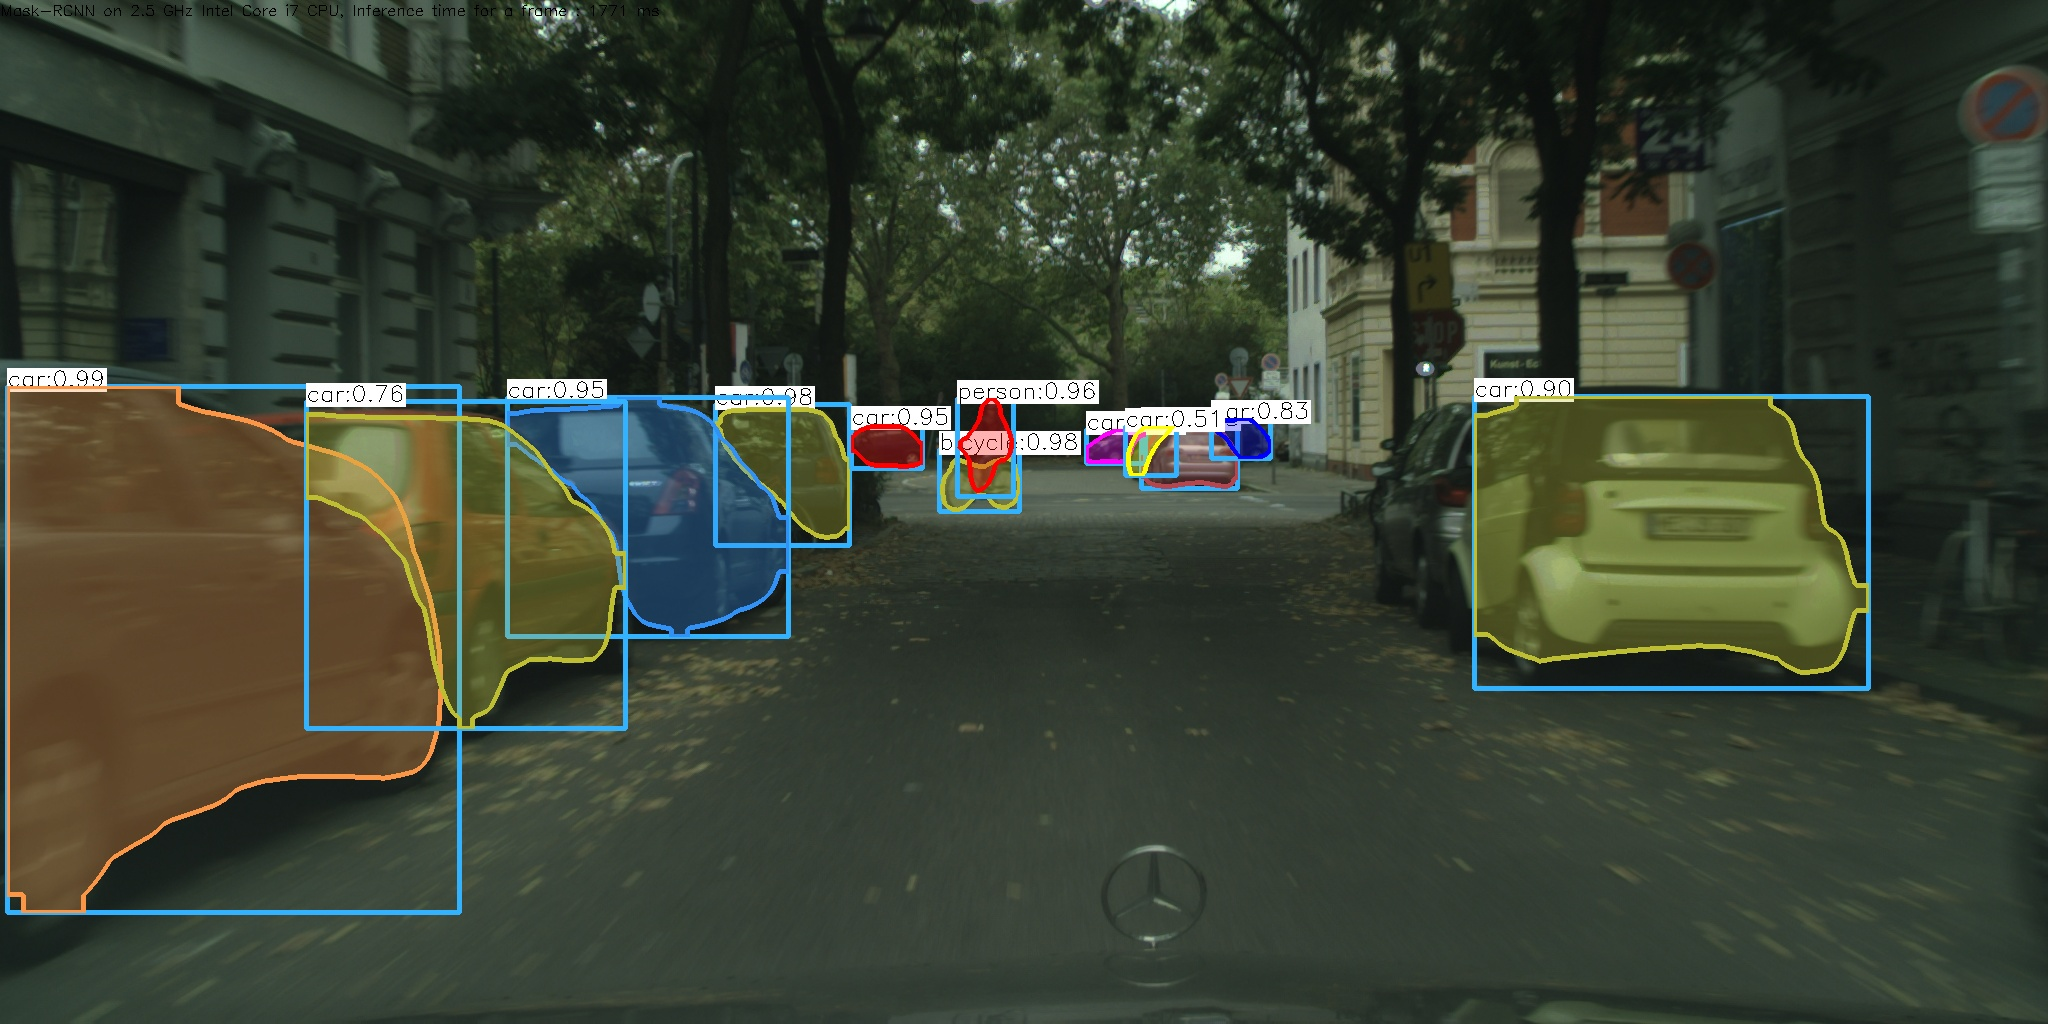
\includegraphics[width=3.7cm, height=1.85cm]{./figure/dusseldorf_000008_000019_leftImg8bit_mask_rcnn_out_py.jpg}}\\ 
			\subfloat{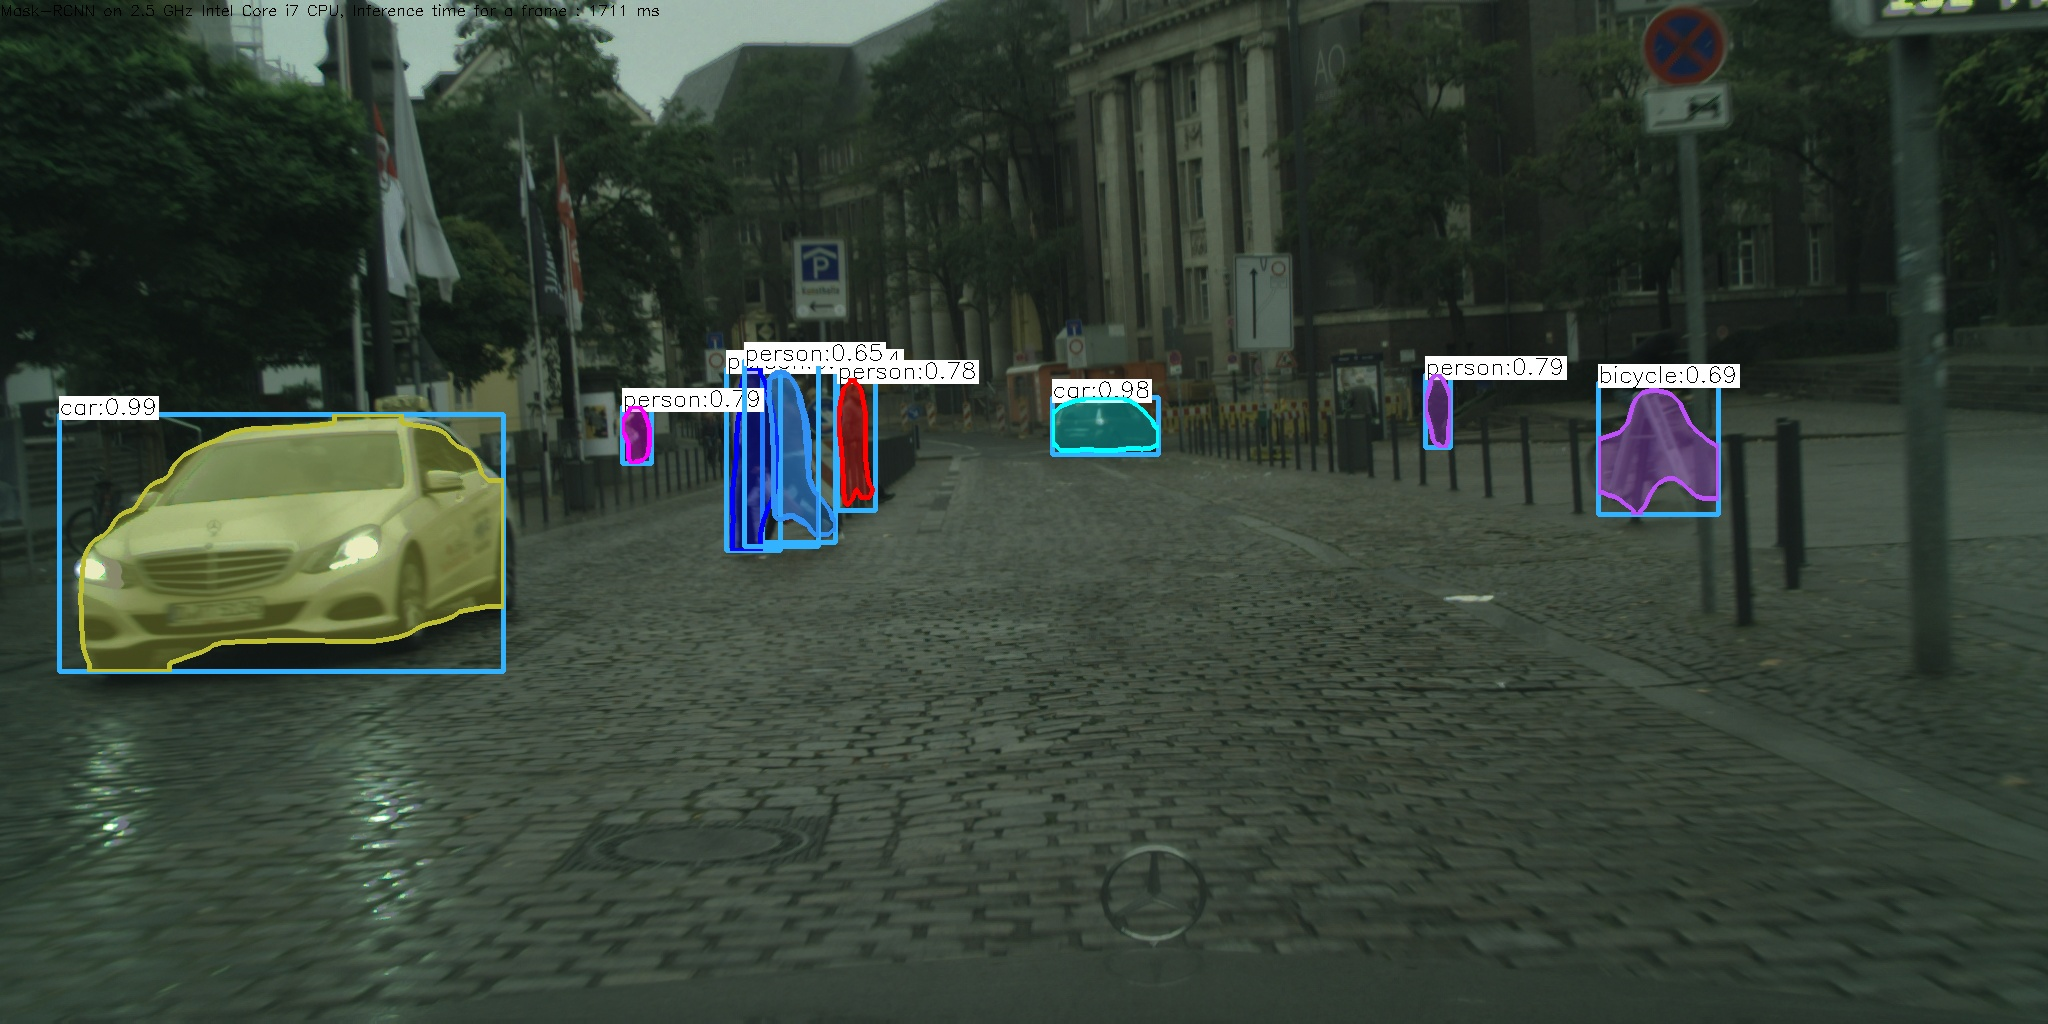
\includegraphics[width=3.7cm, height=1.85cm]{./figure/dusseldorf_000040_000019_leftImg8bit_mask_rcnn_out_py.jpg}}\\
			\subfloat{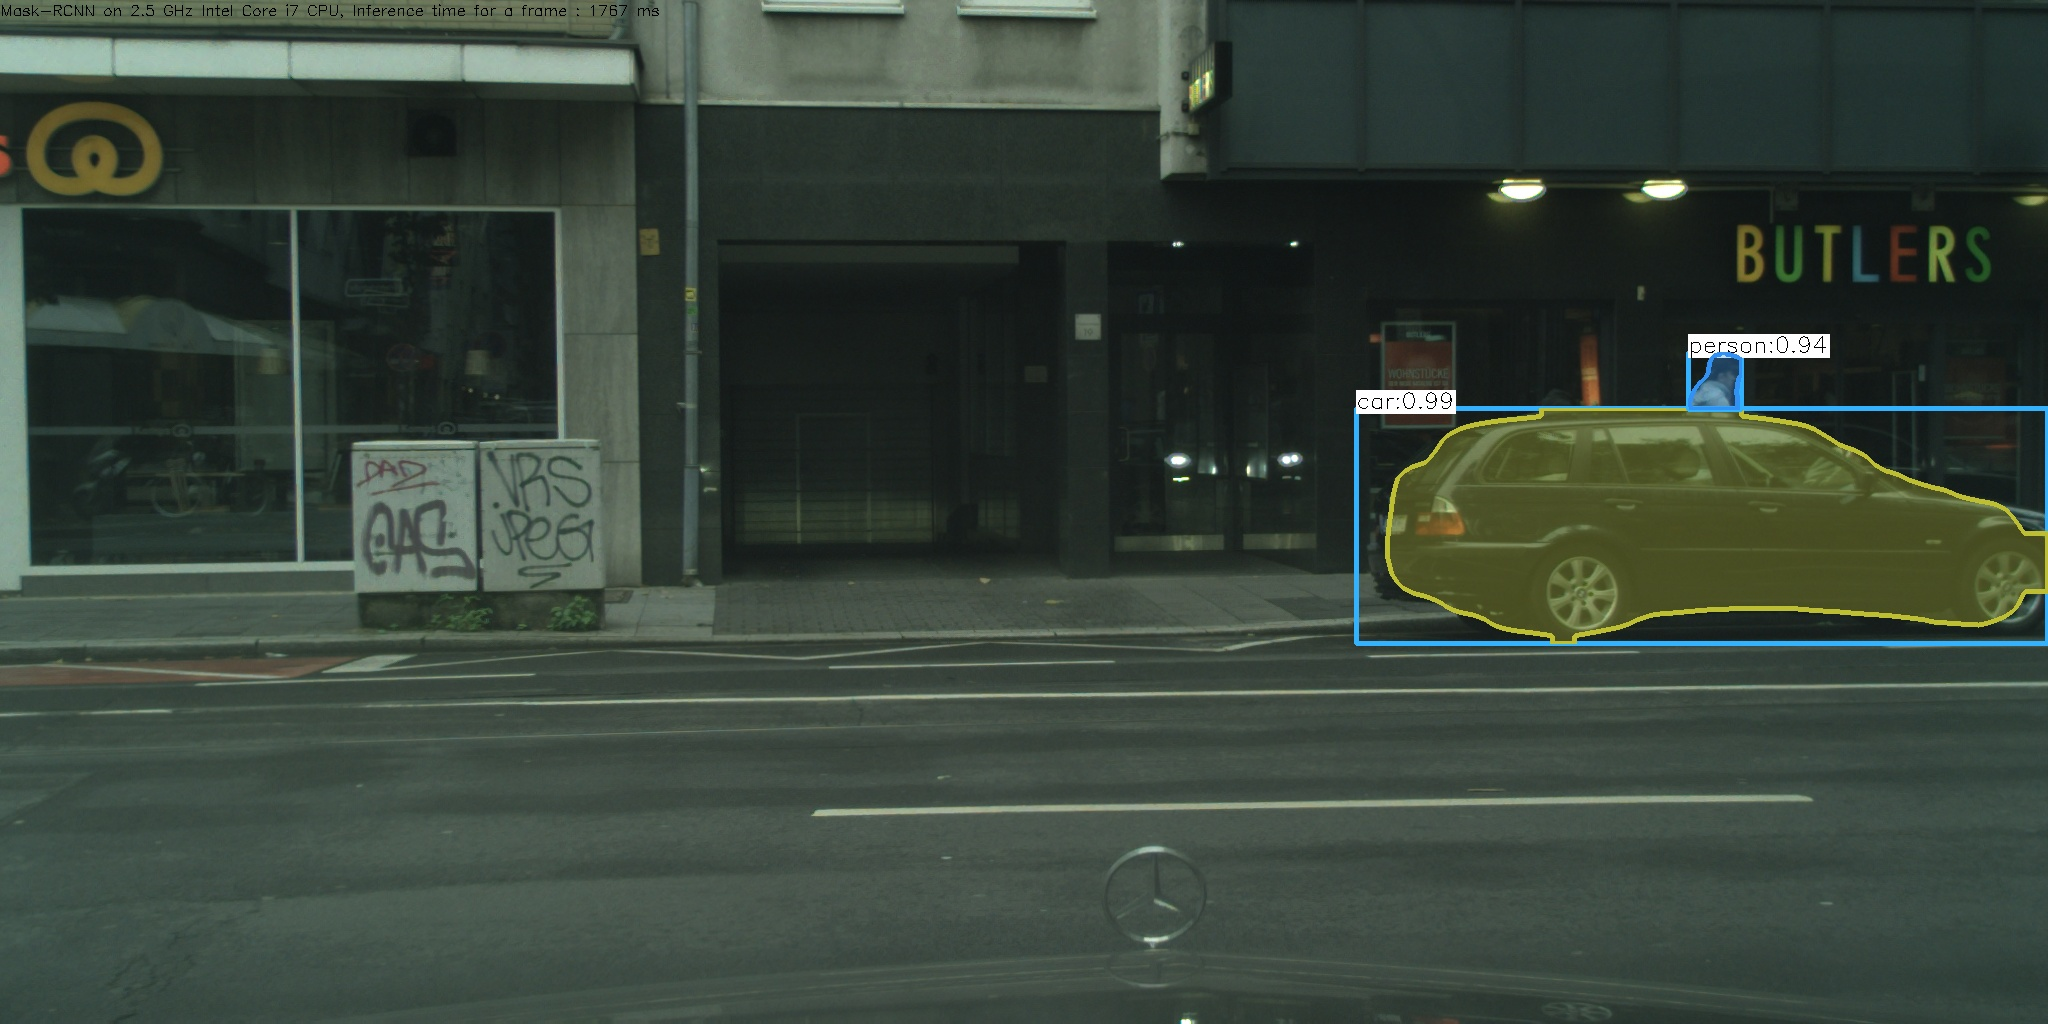
\includegraphics[width=3.7cm, height=1.85cm]{./figure/dusseldorf_000088_000019_leftImg8bit_mask_rcnn_out_py.jpg}}\\ 
			(a) detected cars \cite{rcnn} \\
		\end{tabular}
		&
		\begin{tabular}{cc}
			\subfloat{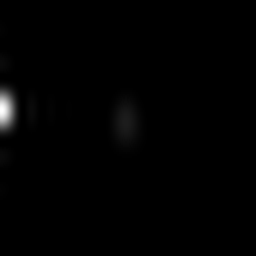
\includegraphics[width=3.7cm, height=1.85cm]{./figure/10_real_A}}\\ 
			\subfloat{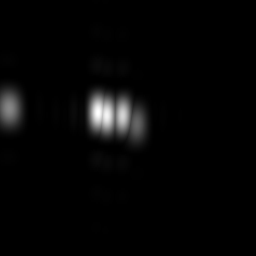
\includegraphics[width=3.7cm, height=1.85cm]{./figure/12_real_A}}\\
			\subfloat{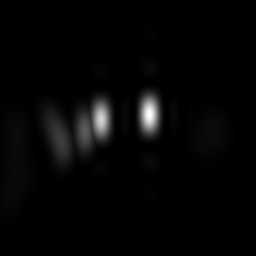
\includegraphics[width=3.7cm, height=1.85cm]{./figure/145_real_A}}\\ 
			\subfloat{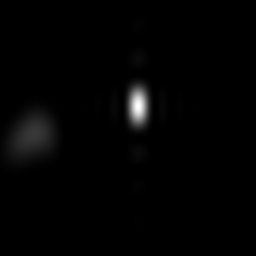
\includegraphics[width=3.7cm, height=1.85cm]{./figure/171_real_A}}\\
			\subfloat{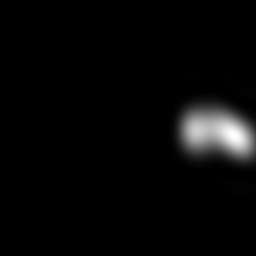
\includegraphics[width=3.7cm, height=1.85cm]{./figure/207_real_A}}\\ 
			(b) input heat-map \\
		\end{tabular}
		&
		\begin{tabular}{cc}
			\subfloat{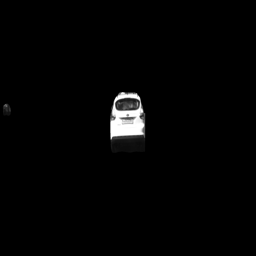
\includegraphics[width=3.7cm, height=1.85cm]{./figure/10_real_B}}\\ 
			\subfloat{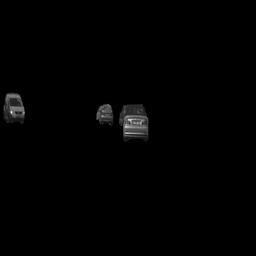
\includegraphics[width=3.7cm, height=1.85cm]{./figure/12_real_B}}\\
			\subfloat{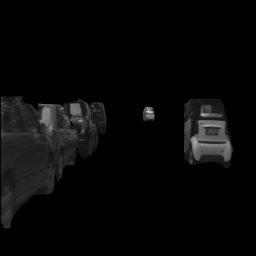
\includegraphics[width=3.7cm, height=1.85cm]{./figure/145_real_B}}\\ 
			\subfloat{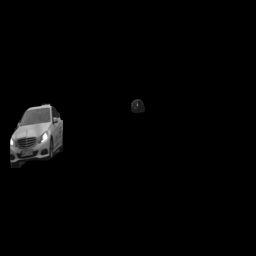
\includegraphics[width=3.7cm, height=1.85cm]{./figure/171_real_B}}\\
			\subfloat{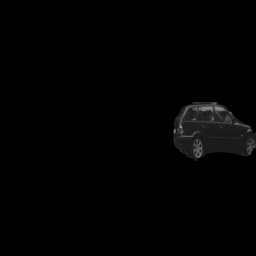
\includegraphics[width=3.7cm, height=1.85cm]{./figure/207_real_B}}\\ 
			(c) ground truth \\
		\end{tabular}
		&
		\begin{tabular}{cc}
			\subfloat{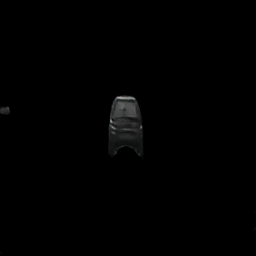
\includegraphics[width=3.7cm, height=1.85cm]{./figure/10_fake_B}}\\ 
			\subfloat{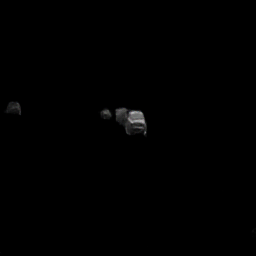
\includegraphics[width=3.7cm, height=1.85cm]{./figure/12_fake_B}}\\
			\subfloat{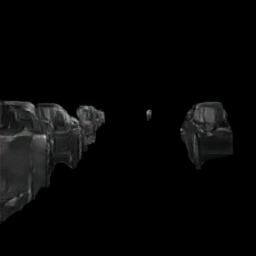
\includegraphics[width=3.7cm, height=1.85cm]{./figure/145_fake_B}}\\ 
			\subfloat{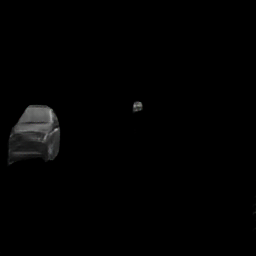
\includegraphics[width=3.7cm, height=1.85cm]{./figure/171_fake_B}}\\
			\subfloat{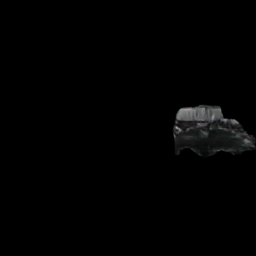
\includegraphics[width=3.7cm, height=1.85cm]{./figure/207_fake_B}}\\ 
			(d) generated image \\
		\end{tabular}
	\end{tabularx}	
	\caption{Some results from the second experiment. From top to bottom: 1) The car's boundary, shape and orientation has fully been recovered. The gray-scale colors do not much. However, colors are of little importance in our application. 2) The orientation of the middle car is reversed. As we shall see in the next section, 180 degrees of ambiguity can easily be fixed using the Doppler effect. 3) Although there is high reflection from the middle car, its boundary has correctly been identified as a small distant car. 4) Same as 3. Also the orientation of car on the side has been correctly estimated. 5) The generated image does not make sense. This is most likely because the sides of cars were rarely included in the training images provided to the network. }\label{fig2}
\end{figure*}
In the second experiment, as mentioned in the dataset section, we synthesized a more realistic dataset that is very similar to radar images. In most cases, the GAN was able to restore the boundaries and the orientation of the cars \ref{fig2}. It has also learned to identify the cars some of whose parts are blocked, either because they appear near the edge of image, or appear behind other cars.

As mentioned before, one significant problem with radar images is that some objects in appear to be much weaker or stronger in power than others, depending on their angle with the receiver mmWave antenna. The results from this experiment show that the GAN is able to learn this phenomenon and compensate for it. As a result, it is able to identify the cars, even if the reflection from them is weak. For instance, in the fourth row of figure \ref{fig2}, the GAN successfully   

